\documentclass{llncs}

\usepackage{amsmath}
\usepackage{graphicx}
\usepackage{amssymb}
\usepackage{color}
\usepackage{wrapfig}
\usepackage{url}
\usepackage{scalefnt}
\usepackage{tikz}
\usepackage{overpic}
\usepackage{multirow}
\usepackage{soul}
\usetikzlibrary{automata,positioning}
\usetikzlibrary{arrows}

%\addtolength{\textfloatsep}{-0.7em}
\newcommand{\INIT}{\STATE \textbf{init} {}}
\newcommand{\df}{\scalebox{.9}{$\stackrel{{\tiny \mathrm{df}}}{=}$}}
\newcommand{\TBA}{{\bf TBA}}

\newcommand{\ptort}[1]{\mbox{$\stackrel{#1}{\rightarrow}\hspace{-.65ex}%
                       \raisebox{.15em}{\scriptsize *}\hspace{.65ex}$}}
\newcommand{\ptot}[1]{\mbox{$\stackrel{#1}{\rightarrow}\hspace{-.65ex}%
                       \raisebox{.15em}{\scriptsize +}\hspace{.65ex}$}}
\newcommand{\pto}[1]{\stackrel{#1}{\rightarrow}}
\newcommand{\ptoprime}[1]{\stackrel{#1}{\rightarrow}\hspace{-1mm}\raisebox{-0.5mm}{$'$}{\,}}
\newcommand{\redmod}[2]{{#1}|_{#2}}
\DeclareMathOperator{\AP}{AP}
\DeclareMathOperator{\Succ}{Succ}
\DeclareMathOperator{\SCC}{SCC}
\newcommand{\abs}[1]{\lvert #1\rvert}
\newcommand{\ks}[1][]{\ensuremath{ \mathcal K_{#1}=(\mathcal P, S_{#1},I_{#1},\to_{#1}, L_{#1})\ }}
%{{{ Mod_M
\renewcommand{\mod}[1][\mathcal K]
{\ensuremath{Fragment_{#1}}}
\newcommand{\modul}[1][\mathcal K]%
{\ensuremath{\mathcal{F}_{#1}}}
%}}}

%{{{ MC(M,As) (\mc structure as.f.)
\newcommand{\mc}[1][\mathcal K]{\ensuremath{\mathcal{C}_{#1}}}
\newcommand{\mcpsi}[1][\mathcal K]{\ensuremath{\mathcal{C}_{#1}^\psi}}
%}}}

%{{{ True, false
\newcommand{\ttrue}{\ensuremath{\texttt{tt}}}
\newcommand{\ffalse}{\ensuremath{\texttt{ff}}}
%}}}
%{{{ assumption function
\newcommand{\as}[1][]{\ensuremath{\mathcal{A}_{#1}}}
\newcommand{\AS}[1][\mathcal K]{\ensuremath{AS_{#1}}}
\newcommand{\ASpsi}{\ensuremath{AS_{\mathcal K}^\psi}}
\newcommand{\asu}{\ensuremath{\mathcal{A}_{\bot}}}
\newcommand{\sas}[1][]{\widetilde{\mathcal{A}}_{#1}}
%}}}
%{{{ temporal operators
\newcommand{\AX}[1][\varphi]{\ensuremath{\mbox{\textbf{AX}\,}#1}}
\newcommand{\EX}[1][\varphi]{\ensuremath{\mbox{\textbf{EX}\,}#1}}
\newcommand{\X}[1][\varphi]{\ensuremath{\mbox{\textbf{X}}#1}}
\newcommand{\AUp}[2][\varphi]{\ensuremath{\mbox{\textbf{A}}({#1}\mbox{\,\textbf{U}\,}{#2})}}
\newcommand{\EUp}[2][\varphi]{\ensuremath{\mbox{\textbf{E}}({#1}\mbox{\,\textbf{U}\,}{#2})}}
\newcommand{\Up}[2][\varphi]{\ensuremath{{#1}\mbox{U}{#2}}}
\newcommand{\AU}[1][\varphi]{\ensuremath{\mbox{\textbf{A}}({#1}_1\mbox{\,\textbf{U}\,}{#1}_2)}}
\newcommand{\EU}[1][\varphi]{\ensuremath{\mbox{\textbf{E}}(#1_1\mbox{\,\textbf{U}\,}#1_2)}}
\newcommand{\U}[1][\varphi]{\ensuremath{#1_1 \mbox{\textbf{U}}#1_2}}
\newcommand{\EF}[1][\varphi]{\ensuremath{\mbox{\textbf{EF}\,}#1}}
\newcommand{\EG}[1][\varphi]{\ensuremath{\mbox{\textbf{EG}\,}#1}}
\newcommand{\AG}[1][\varphi]{\ensuremath{\mbox{\textbf{AG}\,}#1}}
%}}}

\newcommand{\oprav}[1]{{\color{red} #1}}

\newcommand{\VR}{\mathit{VR}}

\usepackage{algorithm}
\usepackage[noend]{algpseudocode}
\usepackage{algpseudocode}
% New definitions
\algnewcommand\algorithmicswitch{\textbf{switch}}
\algnewcommand\algorithmiccase{\textbf{case}}
\algnewcommand\algorithmicassert{\texttt{assert}}
\algnewcommand\Assert[1]{\State \algorithmicassert(#1)}%
% New "environments"
\algdef{SE}[SWITCH]{Switch}{EndSwitch}[1]{\algorithmicswitch\ #1\ \algorithmicdo}{\algorithmicend\ \algorithmicswitch}%
\algdef{SE}[CASE]{Case}{EndCase}[1]{\algorithmiccase\
  #1}{\algorithmicend\ \algorithmiccase}%


  \algblockdefx{FORALLP}{ENDFAP}[2]%
  {\textbf{for all }#1 \textbf{do in parallel} #2}%


%% END MACROS SECTION

\begin{document}

\frontmatter          % for the preliminaries
\pagestyle{headings}  % switches on printing of running heads

\mainmatter
\title{High-Performance Symbolic Parameter Synthesis of Biological Models: A Case Study}
%\title{Parallel SMT-Based Parameter Synthesis with Application to Piecewise Multi-Affine Systems%
%Synthesis of Combined Parmeters for Dynamical Systems%
%from CTL Specifications

\author{Martin Demko, Nikola Bene\v{s}, Lubo\v{s} Brim, Samuel Pastva and David {\v{S}}afr\'{a}nek\thanks{This work has been supported by the Czech Science Foundation grant GA15-11089S.}}
\institute{Systems Biology Laboratory, Faculty of Informatics, Masaryk University\\ Botanick\'{a}~68a,  602 00 Brno, Czech Republic,\\
  \email{\{xdemko,xbenes3,brim,xpastva,xsafran1\}@fi.muni.cz}
}

\maketitle
\begin{abstract}
%\vspace*{-2mm}
% zaujimavost biologickych systemov sposobena parametrami, ktore su casto zavisle
% doteraz schopny odhalovat systemy s nezavislimi parametrami + moznost zadavat rozsirene constrainy v zmysle logiky prveho radu
% nova technika a predstavenie jej pouzitelnosti a uzitocnosti (bez formalnej definicie, dokazov a algoritmov)
% pouzitelnost na zlepsenie vyhladavania bistability v modeli G1/S nieco ...
% pouzitelnost v syntetickej biologie pre ulahcenie  (urychlenie) vyskumu
% mozno - skalovatelnost na represilatore

Complex behaviour arising in biological systems is described by highly parameterised dynamical models.
Most of the parameters are mutually dependent and therefore it is hard and computationally demanding to find admissible parameter values with respect to hypothesised constraints and wet-lab measurements.  
Recently, we have developed several high-performance techniques for parameter synthesis that are based on parallel coloured model checking. 
These methods allow to obtain parameter values that guarantee satisfaction of a given set of dynamical properties and parameter constraints.   
%we present an old idea in the brand new coat for uncertain parameters synthesis with application in biological models. Formerly, we were limited to investigate one parameter per equation only. This fact is overcome by employing new symbolic representation of parameters and their constraints in forms of first-order logic formulae. Thereafter a {\em Satisfiability Modulo Theories} (SMT) solver is used to handle state-space generation on which our {\em parallel coloured CTL model checking} procedure is applied in classic way with few differencies. 
%[Short$|$Concise] description of the method is provided in order to reader could understand the story behind. 
In this paper, we review the applicability of our techniques in the context of biological systems.
In particular, we provide an extended analysis of a genetic switch controlling the regulation in mammalian cell cycle phase transition and a synthetic pathway for biodegradation of a toxic pollutant in \emph{E. coli}.
%Every system could be described in terms of some model (e.g., {differential equations}), but some of its quantitative aspects are hard to be measured.
%nature is the reason why all aspects of such a system cannot be precisely quantified (i.e., measured). 
%We are talking about {uncertain parameters} which have direct impact on a particular system's behaviour. In particular, these parameters and their investigation are the main objectives of this thesis proposal.

%In general, there are many approaches for investigation of biological systems properties and their parameters. The topic of the proposed thesis focuses on verification of such properties by model checking, a formal technique originally designed for the analysis of computer systems. Examined properties are defined in terms of {temporal logics} allowing to describe system behaviour over time. However, biological systems are not designed for direct application of such a technique. Therefore there are various methods dealing with this issue. We present an overview of the most common ones and discuss their benefits and drawbacks in order to improve our own proposed approach.

\end{abstract}

\enlargethispage{6mm}
%\vspace*{-3mm}
\section{Introduction}
\label{sec:intro}

%TBA biological problems, and the need for parameter synthesis...

Dynamical models in systems and synthetic biology are typically represented in terms of systems of ordinary differential equations (ODE). These models are quantitative and their functionality relies on adequate selection of parameter values. Practical parametric identification~\cite{Raue} is in many cases the only solution to obtain parameter values that fit with experimental observations.  Due to the limited resolution of wet-lab experimentation, the task is hard. On the other hand, formal methods provide techniques that allow global analysis of model dynamics under uncertainty of parameter values. \emph{Parameter synthesis} is a technique that allows identification of parameter values with respect to a given set of \emph{a~priori} known hypotheses (or requirements) on systems dynamics and parameter constraints (e.g., correlations of parameter values, constraints on production/degradation ratio, etc.).         

There are several levels of complexity that
significantly affect the tractability of parameter synthesis for biological
models. First, the procedure requires consideration of all possible settings of
parameters -- points in the parameter space. The size of the parameter space grows
exponentially with the number of unknown parameters. 
 Second, the complexity of the procedure increases with the number of dependencies among individual parameters. Parameter synthesis methods based on model checking or monitoring systems dynamics are capable to deal with parameter dependencies to some extent. On the contrary, traditional parameter estimation methods that search for an optimal fit of the parameters wrt the given data do not directly deal with dependent parameters~\cite{Raue} (manual work is required -- model reduction or reformulation). 

 %during each model
%checking phase -- analysis of the model with particular parameter settings --
%the dynamics of the model has to be explored. More precisely, the state space of
%the model, which grows exponentially with the number of state variables, has to
%be traversed in each model checking phase. 

Several methods and tools based in computer science have been developed to tackle advanced analysis of biological models~\cite{reviewEzio16}. Given the complexity of the problem and the need for comprehensive large-scale
models, there is a natural call for development of techniques prepared to
perform efficiently on high-performance computing
platforms~\cite{BGMP09}. 
The complexity caused by the state space and parameter space size can be reduced by parallel techniques. The achieved efficiency is
again highly dependent on the modelling approach, the nature of models, and the
properties considered. %In the case of biological models, symbolic techniques
%were successfully employed for abstract logical (qualitative)
%models~\cite{BattPCGMJ10,FagesS08} whereas enumerative parallel techniques have proved to be
%fruitful for quantitative models~\cite{BGMP09,BBS10}.

In this paper, we formulate a general framework for parameter synthesis using several recently developed techniques based on model checking~\cite{CMSB15,TCBB,ATVA}.
In particular, these techniques work with a given Computational Tree Logic (CTL) specification of behaviour constraints and a given initial parameter space (potentially refined with \emph{a~priori} known constraints on parameter values). In this context, parameter synthesis is solved by the coloured model checking technique extended with symbolic encoding of parameter valuations. The paper focuses primarily on case studies and practical evaluation of the workflow. As a part of the workflow, we apply a recently developed parallel algorithm published in~\cite{ATVA}.

The contribution of this paper is a general workflow for parameter synthesis based on model checking and application of this workflow to two different biological case studies that are of high importance in systems and synthetic biology. In particular,  we provide an extended analysis of a genetic switch controlling the regulation in mammalian cell cycle phase transition and a synthetic pathway for the biodegradation of a toxic pollutant in \emph{E. coli}.

\enlargethispage*{5mm}
\paragraph{Related Work.}
Existing techniques for parameter synthesis from temporal specification are either based on model checking performed directly over a qualitative finite quotient of systems dynamics~\cite{BYW+07,YB08,TCBB,CMSB15}, on techniques from hybrid systems~\cite{Bogomolov15}, and on polytopic set representations employed with on-the-fly refinement of the parameter space~\cite{Dang2015}. Our technique can be treated as an extension to the first group of techniques. By employing SMT, we obtain a general framework that supports all parameterisations and constraints that can be encoded in a first-order logic over reals. Techniques in~\cite{BYW+07,GrosuBFGGSB11} also fit our workflow well, they encode parameter sets symbolically in terms of polytopes allowing to capture linear dependencies. To the best of our knowledge, the mentioned related techniques have not been parallelised yet.

Monitoring-based techniques~\cite{RBF+09,DonzeBreach} have an advantage that the function defining the systems dynamics is considered as a black box provided that there is basically no limitation on the form of parameterisation. A significant advantage of these techniques is the ability of quantitative analysis giving detailed insights on the sampled parameter space. In our workflow, we employ these methods in the post-processing phase. 
Additionally, a promising fact is that numerical solvers can be replaced with SMT solvers for non-linear functions and real domains~\cite{GaoKC13,BioPsy}. However, these techniques currently focus on reachability analysis only and their extension to general temporal specifications is a non-trivial task yet to be explored as well as their inclusion into the overall model-checking-based parameter synthesis framework. 

% The main principle of our method relies on symbolic representation of
% coloured transition relation by means of first-order formulae encoding the
% respective colours under which the transition relation is valid. More
% specifically, existence of a particular transition is reduced to satisfiability
% of the formula encoding the respective parameter valuations enabling the
% transition. The parameter encoding relies on the first-order theory of reals for
% which the satisfiability can be algorithmically solved~\cite{Basu06}. In
% particular, we employ \emph{Satisfiability Modulo Theories} (SMT) as a
% subprocedure wrapped inside the enumerative CTL model checking algorithm. This
% allows for every state to synthesise a first-order formula that encodes the
% parameter valuations for which the CTL specification is guaranteed to be
% satisfied in that state. A significant advantage of employing enumerative CTL model checking for
% parameter synthesis is its capability of computing integrated information in a
% single run. In particular, the parameter valuations are synthesised for every
% state and every subformula of the given CTL property. This allows to compute the
% parameter synthesis for a set of CTL formulae in a single run.

% In:http://bioinformatics.oxfordjournals.org/content/31/12/i89.full.pdf

% Reconstructing gene regulatory dynamics from
% high-dimensional single-cell snapshot data
% Andrea Ocone1
% , Laleh Haghverdi1
% , Nikola S. Mueller1
% and
% Fabian J. Theis1,2,*

%Complex dynamical phenomena arising in real-world systems such as biological,
%biophysical processes or networks involving economic and social interactions are
%typically formalised by means of \emph{dynamical systems} employing the framework of non-linear ordinary differential equations or difference equations that are highly
%parameterised. In most cases, the model complexity and number of \emph{unknown parameters} do not allow to analyse the models analytically and therefore the
%analysis is often restricted to numerical and statistical methods.
%
%Phenomena occuring in the time domain of systems dynamics can be efficiently encoded in \emph{temporal logics} (TL). TL have the advantage of rigorous and abstract representation of sequences (or even branching structures) of desired observable events in systems dynamics including quantitative bounds on time and variable values~\cite{STL,STL*,BYW+07} and can be also combined with frequency-domain analysis~\cite{TFL}. Computer-aided analysis of complex dynamical systems and their models is a necessary precursor for design of reliable cyber-physical and cyber-biological systems such as synthetic design and control of living cells~\cite{Khammash,Dvorak2015} or safe medical treatment~\cite{Oleg}. 
%
%In general, computationally efficient (scalable) global analysis of systems dynamics under large uncertainty of a number of unkown parameters and unrestricted initial conditions with respect to satisfaction of a given TL specification remains a challenge. Existing techniques do not sufficiently target non-quantitative branching-time properties that can efficiently cope with \emph{decision} events and \emph{multi-stability} arising in complex real-world systems (e.g., unstable states in chemical or electric power systems~\cite{Li15,Chiang16}, or reachability of multiple stable states in a biological switch~\cite{switch,SKH04}). It is also worth noting that it is often necessary to incorporate all known constraints on parameters since they may significantly reduce the extent of parameter uncertainty. Several recent case studies~\cite{Theis2015,Schneider2013,Dvorak2015} have shown that many additional parameter constraints are often known \emph{a~priori} and therefore parameter synthesis methods should be able to reflect them in the workflow.
%
%In this paper, we target the problem of \emph{global parameter synthesis} (extended with \emph{static constraints} over parameter space). To solve the problem means to \emph{identify parameter valuations} that \emph{satisfy} a given set of \emph{TL properties} universally (regardless specific initial conditions) and also \emph{satisfy} the specified \emph{static constraints}.
%
%Our contribution is a novel approach to global parameter synthesis that is based on model checking with respect to CTL specification and symbolic representation of parameter constraints in terms of first-order formulae over real variables that are sufficiently handled with SMT solvers. In particular, parameter synthesis for a given CTL specification and the given parameter space is solved by coloured model checking technique extended with symbolic encoding of parameter valuations. The \emph{parametrised dynamical system} is represented as a \emph{family of state-transition systems} that share the same state space but differ in \emph{transition relations} that are distinct for particular parameter valuations (we say transitions are \emph{coloured} provided that every parameter valuation is considered as a transition relation of a distinctive colour). %In particular, every parameter valuation is considered as the transition relation of a respective fixed colour. 
%The main principle of our technique relies on symbolic representation of coloured transition relation by means of parameter constraints encoding the respective colours under which the transition relation is valid. More specifically, existence of a particular transition is reduced to satisfiability of the formula encoding the respective parameter constraints enabling the transition. The satisfiability is solved by SMT. As a subprocedure, it is wrapped inside the enumerative CTL model checking algorithm that synthesises for every state a first-order formula that encodes the parameter valuations for which the CTL specification is guaranteed to be satisfied in that state.
%
%Our method is unique in combining enumerative model checking with SMT. It is distinctive in the following aspects:
%\begin{enumerate}
%\item universality -- method works on a large family of finite-state discrete dynamical systems or finite-state qualitative abstractions of continuous systems in which parameterisations can be encoded in a first-order logic over reals,
%\item user feedback -- resulting parameter sets are sampled from the SMT representation and further post-processed by third-party tools such as Symba~\cite{Li15},
%\item high-performance -- the method is supplied with a parallel distributed-memory algorithm that allows good scalability in a distributed environment.
%\end{enumerate}
%
%The typical application domains are highly parametrised systems appearing in systems biology (e.g., dynamics of gene regulatory networks represented by boolean networks or non-linear continuous systems~\cite{BattPCGMJ10}) or control and verification of hybrid systems~\cite{Donze2009}. In this paper, we consider a case study on dynamical systems of gene regulatory networks.
%
%Universality of the proposed method is limited in the complexity of considered parameter constraints and the respective efficiency of SMT solvers. In the case study, we apply the method to piece-wise multi-affine dynamical systems (PWA) where the systems dynamics is a linear function of the parameters. Under this setting, the parameters are allowed to form linear combinations. As static constraints we consider any constraints for which satisfiability is decidable and effectively computable. In our case study, we are interested in constraining the ratio of particular parameters, in particular, fine-tuning of protein production/degradation rate ratio is of high importance in synthetic biology~\cite{Rosenfeld2003}. 
%
%A significant advantage of emloying enumerative CTL model checking for parameter synthesis is its capability of computing integrated information in a single run. In particular, the parameter valuations are synthesised for every state and every subformula of the given CTL property. This allows to compute the parameter synthesis for a set of CTL formulae in batch.     
%
%Distributed algorithm is based on assumption-based CTL model checking we have introduced in~\cite{BrimYZ05}. Its extension to parameter synthesis for interval-representation of parameter sets has been introduced in~\cite{CMSB15}. The main drawback of that approach has been restriction to synthesis of algebraically independent parameters. By using SMT, we significantly generalise the method to parameterisations including interdependent parameters. The new algorithm retains good scalling with increasing number of computing nodes. % and fights the size of the state space and number of unknown parameters. 
%Since the number of calls to an SMT solver is proportional to the size of the state space, distribution of the state space and related computing tasks realises efficiently the divide\&conquer paradigm while minimising the number of SMT calls and parallelising their computation on independent computing nodes.  
%%rozdelit graf stavoveho prostoru na mensi kousky se z3 - rozdel a panuj
%%intro motivace - ne nutne z3 ale obecne procedura SMT trva ... zmenseni grafu .. redukujeme pocet volani solveru...nezavisle vypocty
%
%%CTL
%%Our approach that allows those properties: enumerative CTL model checking with SMT


%\subsection{Related Work}
%
%Monitoring-based synthesis techniques have been developed for continuous-time and discrete-time dynamical systems~\cite{RBF+09,DonzeBreach,STL*,BBS10,Raman15} and linear-time TL.
%These techniques rely on numerical solvers which are well-developed for systems with fixed parameters or small parameter spaces (perturbations). An advantage of these techniques is that they consider the function defining the systems dynamics as a black box provided that there is basically no limitation on the form of parameterisation of the system. The main drawback is the need to sample the parameter space and initial states while loosing robust guarantees for the results. This drawback can be overcome by replacing numerical solvers with Satisfiablity Modulo Thories (SMT) solvers that can cope with non-linear functions and real domains up to required precision~\cite{GaoKC13}. However, these techniques are limited to reachability analysis~\cite{BioPsy} and their extension to work with general TL specifications is a non-trivial task yet to be explored.
%
%Existing techniques for global parameter synthesis address the solution only partially. They are either based on model checking performed over a qualitative finite quotients of systems dynamics~\cite{BYW+07,YB08,TCBB,CMSB15} or they employ techniques from hybrid systems analysis~\cite{Bogomolov15}. In all those cases, the systems dynamics cannot be considered as a black box. The main limit is given by restrictions imposed on the form of allowed model parameterisations. Typically, the system dynamics is required to be a linear function of the parameters. However, in practise this limitation is often violated (e.g., enzyme kinetics, competitive and non-competitive interactions in genetic networks, etc.) 

%TBA compare to algebraic techniques of Carla etal.

%A well-established solution is based on statistical approaches~\cite{Clarke_SMC,Sen_SMC,BortolussiS14}. The methods typically involve clever ways of sampling which is still computationally demanding when it comes to large dimensionality of systems uncertainty (number of samples needed in general increases exponentionally with number of uncertain parameters). To gain the most important advantages of formal methods, it is necessary to be able to analyse models of systems dynamics in any theoretically possible initial state and to obtain a guaranteed set of parameter values under which the required phenomenon is achieved. In statistical methods, this aspect is approached within confidence bounds.

%Existing methods ranging from likelihood-based parameter estimation through sensitivity analysis to bifurcation analysis give results
%only within a computed statistical confidence. Morever, numerical methods allow only local analysis regarding the initial conditions. However, it is often important to analyse the system dynamics in any theoretically possible initial state and to obtain a precise set of parameters where the studied phenomenon is guaranteed.




% \textit{The goodness of fitting for favoured models is also reflected in estimated
% parameter values. Parameter posterior distributions are reported in Figure 3,
% together with true parameters used to simulate snapshot data. Average of
% relative errors, computed using maximum a posteriori estimates, is around
% 17\%. However, parameter estimation performance is mixed: mode of posterior distributions for some
% parameters is very close to true values, whereas for other parameters, such as
% Hill coefficients h, it is not as good. Variations of Hill coefficients h
% determine only small changes in the slope of $g_z$ expression overshoot, therefore
% even small error sources in gene expression values or pseudo time reconstruction
% make estimation of h nontrivial. Plots of bivariate marginal distributions
% (Fig. 3, left) show high correlation between parameters $\alpha$ and $\lambda$. Although we are
% not able to recover their true values, nonetheless the ratio between their
% posterior estimates is exactly the true one (Fig. 3, right,True parameters ratio
% is given by $\alpha / \lambda =400$). }

% a take se podivat na: http://www.ncbi.nlm.nih.gov/pmc/articles/PMC3643600/

% TBA: scalability

% TBA: CAV for complex systems...cite something...why guarantees are
% useful...mention methods that proved to be good

% To capture biologically-relevant temporal hypotheses both branching-time
% operators and linear-time operators are needed~\cite{Batt05validationof}. In
% this paper we focus on \emph{branching logic} CTL. The reason is there are many
% important phenomena in systems biology that can be sufficiently expressed only
% by employing branching operators. E.g., switching mechanisms and multi-stability
% are present in genetic regulatory networks and drive many key biological
% phenotypes such as, e.g., irreversible decisions in cell division, cell
% differentiation or programmed cell death. In case of such properties, it is
% difficult (or often impossible) to express relevant properties in linear
% temporal logics. Other reason for usage of CTL is related to the particular
% (enumerative) procedure for coloured model checking. This procedure inherently
% identifies all system states (and parameters) where the given property is
% satisfied. It leads inherently to global analysis of systems dynamics.

% Several methods for parameter synthesis based on model checking have been
% proposed recently, targeting different kinds of models and different temporal
% logics (e.g.,~\cite{TCBB,BattPCGMJ10,Gilbert,DonzeCL10,Jha2011}). In~\cite{TCBB}
% we proposed a parameter synthesis method for LTL hypotheses established on
% automata-based \emph{colored} LTL \emph{model checking}
% algorithm. In~\cite{CMSB15}, we have brought the coloured model checking
% technique to CTL logic by adopting enumerative distributed CTL model checking
% algorithm.


\section{Methods}
\label{sec:methods}

The overall procedure of parameter synthesis based on model checking consists of several tasks. The general overview of the workflow is depicted in Fig.~\ref{fig:workflow} (left).
In particular, the input of the method is a set of \emph{behaviour constraints} specifying requirements on the systems dynamics, a set of \emph{parameter constraints} collecting all \emph{a~priori} known restrictions, dependencies and correlations of individual parameter values, and finally, a dynamical system represented as a potentially non-linear system of ordinary differential equations (\emph{ODE model}).  


The workflow can be realised with any parameter synthesis method based on model checking and discretisation of the input ODE model by means of qualitative finite quotient rigorously abstracting its dynamics. In our case, we employ the technique of \emph{coloured model checking} that provides a single-run heuristics to exploration of the parameter space wrt the given behaviour constraints. The output of the method is a collection of sets of parameter values for which the given behaviour and parameter constraints are guaranteed to be satisfied. This result can be further post-processed. First, the~SMT-based optimisation tools such as Symba~\cite{LiA15} can be used to find approximate parameter values optimal with respect to a given objective function. Second, sampling or statistical model checking can provide detailed exploration of the valid parameter space including quantitative measures such as satisfaction degree~\cite{RBF+09}. All the steps starting from approximation, abstraction and finally the parameter synthesis are automatised by the respective algorithms. The only input required from the user (in addition to the models and constraints) is a parameter setting the precision of the approximation step. Finally, to automatise processing and visualisation of the resulting data, we have implemented a set of scripts written in the R language.  

An important fact is that simulation results performed on the ODE models can be aligned with model checking results only approximately due to the different nature of approximation errors occurring in both methods. To explore the resulting space by monitoring while correctly aligning the results with model checking, the simulation has to be performed on the approximated (PMA) model.

\begin{figure}
\begin{center}
\includegraphics[width=\textwidth]{workflow.pdf}
\vspace*{-1cm}
\end{center}
\caption{Overall workflow of parameter synthesis for ODE models based on model checking (left). Refined description of the coloured model checking procedure for the case of SMT-based symbolic representation of parameter sets (right).}  
\label{fig:workflow}
%\vspace*{-4mm}
\end{figure}
\enlargethispage*{8mm}

\paragraph{Model.}
Let $\mathbb{P}\subseteq \mathbb{R}^m_{\geq 0}$ denote the \emph{continuous parameter space} of dimension $m$.
A~\emph{biological model}
%-- an ODE model to which the workflow can be applied --
has to be given as a~system of ODEs of the form $\dot x = f(x, \mu)$ where $x = (x_1, \ldots, x_n)\in\mathbb{R}^n_{\geq 0}$ is a~vector
of variables, $\mu = (\mu_1, \ldots, \mu_m)\in\mathbb{P}$ is a~vector of parameters,
and $f = (f_1, \ldots, f_n)$ is a~vector where each component is a function constructed as a sum of reaction rates where every sum member represents an affine or bi-linear function of $x$, or a sigmoidal function of $x$. In particular, this restriction covers mass action kinetics with stoichiometric coefficients not greater than one and any sigmoidal kinetics such as all significant variants of enzyme or Hill kinetics. An important additional requirement is that each $f_i$ must be affine in $\mu$.

\paragraph{Constraints.} 
To express \emph{behaviour constraints} of interest, we employ the standard branching time logic
CTL. The formulae of CTL are defined by the following abstract syntax:
\[ \varphi ::= q \mid \neg\varphi \mid \varphi_1\wedge\varphi_2
	\mid \AX \mid \EX \mid \AU \mid \EU \]
where $q$ ranges over the atomic propositions from the set $\AP$.
We use the standard abbreviations such as $\EF \equiv \EUp[\ttrue]{\varphi}$
and $\AG \equiv \neg \EF[\neg\varphi]$.

To express initial \emph{parameter constraints} on the admissible parameter space, we employ a quantifier-free formula with parameters at the place of variables and inequalities at the place of predicates, denoted as $\Phi_I$.  

\paragraph{Approximation.} 
We consider dynamical systems $\dot x = f(x, \mu)$ satisfying the criterion that every $f_i$ is piecewise multi-affine (PMA) in $x$. To achieve that we employ the approach defined in~\cite{GrosuBFGGSB11}. In particular, each sigmoidal function member in $f_i$ is approximated with an optimal sequence of piecewise affine ramp functions. In this procedure, a finite number of thresholds is introduced for every component of $x$. %A cumulative \emph{approximation error} characterising the distance of the approximation from the original function can be computed. 
The crucial factor of the approximation error is the number of piecewise affine segments.
%An example of approximation error for Michaelis-Menten kinetics is shown in Table~\ref{tab:approx-error}.

%\begin{table}
% \center
% \setlength{\tabcolsep}{5pt}
% \begin{tabular}{ |{c}|*{6}{c|} }
%    \hline
%	 & 5  & 6 & 7 & 8 & 9 & 10 \\ \hline \hline
%%%%% Table for: AG low || AG high
%%	100 & 0.000509106  & 0.000275155 & 0.000143549 & 0.000084158 & 0.000057779 & 0.000037046 \\ \hline
%	100 & 5.0911e-04  & 2.7516e-04 & 1.4355e-04 & 8.4158e-05 & 5.778e-05 & 3.7046e-05 \\ \hline
%	200 & 5.1106e-04  & 2.7773e-04 & 1.4472e-04 & 8.5761e-05 & 5.5147e-05 & 3.5036e-05 \\ \hline	
%	400 & 5.1116e-04  & 2.7686e-04 & 1.4484e-04 & 8.5535e-05 & 5.5179e-05 & 3.4975e-05 \\ \hline
%  \end{tabular}
%  \caption{Cummulative approximation error for a Michaelis-Menten function. Individual columns represent different numbers of requested ramp segments. In the rows, particular numbers of evaluation points were selected. Note the increasing number of evaluation points does not notably reduce the error while the number of segments remains the crucials factor.}
%  \label{tab:approx-error}
%\end{table}

\paragraph{Abstraction.}
We employ the rectangular abstraction~\cite{BYW+07,GrosuBFGGSB11}.
We assume that we are given a~set of thresholds $\{\theta^i_1, \ldots,
\theta^i_{n_i}\}$ for each variable $x_i$ satisfying $\theta^i_1 < \theta^i_2 <
\cdots < \theta^i_{n_i}$.  Each $f_i$ is assumed to be multi-affine on each
$n$-dimensional interval $[\theta^1_{j_1}, \theta^1_{j_1+1}] \times \cdots
\times [\theta^n_{j_n}, \theta^n_{j_n+1}]$. We call these intervals rectangles.
Each rectangle is uniquely identified via an~$n$-tuple of numbers: %as follows:
$ R(j_1, \ldots, j_n) = [\theta^1_{j_1}, \theta^1_{j_1+1}] \times \cdots \times
[\theta^n_{j_n}, \theta^n_{j_n+1}] $, where the range of each $j_i$ is $\{ 1,
\ldots, n_i - 1 \}$. We also define $\VR(j_1, \ldots, j_n)$ to be the set of all
vertices of $R(j_1, \ldots,
j_n)$. %The set $F_i(j_1,...,j_n)=[\theta_{j_1}^1,\theta_{j_1+1}^1]\times ...\times \theta_{j_i}^i

% In order to establish a finite rectangular abstraction of the PWMA model,
% special care has to be given to boundary rectangles. A boundary rectangle is any
% rectangle $R(j_1,...,j_n)$ where for some $i$ either $j_i=1$ or $j_i=n_i-1$. Any
% dimension~$i$ satisfying that condition is called a boundary dimension of
% $R(j_1,...,j_n)$. We restrict ourselves to models where the dynamics is bounded
% in the range specified by lower and upper thresholds -- trajectories cannot exit
% that range (note that this could occur only in boundary rectangles). Formally,
% all trajectories determined by the PWMA model are required to keep $x_i\in
% [\theta_1^i,\theta_{n_i}^i]$. We restrict ourselves to parameter spaces where
% this requirement is satisfied for all parameter values. More precisely, for
% every boundary rectangle $R(j_1,...,j_n)$ we assume that for all
% $\mu\in\mathbb{P}, i\in\{1,...,n\}, x\in R(j_1,...,j_n)$ it holds that
% $(j_i=1\wedge x_i=\theta_1^i) \Rightarrow f_i(x,\mu)>0$ and $(j_i=n_i-1\wedge
% x_i=\theta_{n_i}^i)\Rightarrow f_i(x,\mu)<0$.

It has been shown that rectangular abstraction is conservative with respect to almost all trajectories of the original (continuous) PMA model~\cite{Batt2007}. %In particular, almost every continuous trajectory in the PWMA model is covered by a corresponding sequence of rectangles in its rectangular abstraction. However, there may exist a sequence of rectangles for which there is no corresponding continuous trajectory in the original PWMA model.
The rectangular abstraction results in a state-transition system, a so-called \emph{parameterised Kripke structure}, defined as $\mathcal{K}=(\mathbb{P},S,\rightarrow,L)$ with $S = \{ (j_1, \ldots, j_n) \mid \forall i : 1 \le j_i \le n_i \}$ where each $\alpha \in S$ represents the rectangle $R(\alpha)$.  The atomic propositions representing concentration inequalities are assigned to adequate states by means of the labelling $L$. In particular, $L: S\rightarrow 2^{AP}$ where 
$AP=\{x_i\odot\theta^i_j\mid 1\leq i\leq$ $n,1\leq j\leq n_i\},\odot\in\{\leq,\geq\}\}$. The transition relation $\rightarrow$ is defined between any two states representing adjacent rectangles. Each transition is associated with a subset of parameter values under which it is allowed. %Its detailed description is provided in the next paragraph.

\paragraph{Symbolic Encoding of Parameters.}

Let now $\alpha = (j_1, \ldots, j_n) \in S$, $1 \le i \le n$ and $d \in \{-1, +1\}$.
We define $\alpha^{i,d} = (j_1, \ldots, j_i + d, \ldots, j_n)$
(if $j_i + d$ is in the valid range). Thus $\alpha^{i,d}$ describe all
the neighbouring rectangles of $\alpha$.
We further define
$v^{i,+1}(\alpha) = \VR(\alpha) \cap \{ (..., j_i+1, ...) \}$ and
$v^{i,-1}(\alpha) = \VR(\alpha) \cap \{ (..., j_i, ...) \}$.
To define the transition relation $\rightarrow$ of the parameterised Kripke structure $\mathcal K$, every pair of states $\alpha,\alpha^{i,d}\in S$, $1\leq i\leq n$, $d\in\{-1,1\}$, is associated with a formula $\Phi_{\alpha,\alpha^{i,d}}$ symbolically encoding the set of parameter values $\mu\in\mathbb{P}$ for which the transition $\alpha\rightarrow\alpha^{i,d}$ is valid:

%For $\alpha$, $\beta in S$, we say that $\alpha$ is connected to $\beta$
%of $\alpha \ne \beta$ and there exists $1 \le i \le n$ and $d \in \{-1, +1\}$
%such that $\alpha_i = \beta_i + d$ and for all $1 \le j \le n$, $i \ne j$,
%$\alpha_i = \beta_i$. We denote this by $\alpha \xrightarrow{i} \beta$ if
%$d = +1$, $\beta \xrightarrow{i} \alpha$ otherwise.
%
%Let $\alpha \xrightarrow{i} \beta$. The common corners of $\alpha$ and $\beta$,
%denoted by $corners(\alpha,\beta) = \{ (\theta^1_{x_1}, \ldots, \theta^n_{x_n})
%\mid x_i = \beta_i$ and $\forall j \ne i : x_j \in \{\beta_j, \beta_j+1\} \}$.
%
%The transitions in the rectangular abstraction system for connected
%rectangles $\alpha \xrightarrow{i} \beta$ are defined as follows:
%
%\begin{align*}
%\varphi_{\alpha,\beta} &:= \bigvee_{v \in corners(\alpha,\beta)} f_i(v,\mu) > 0\\
%\varphi_{\beta,\alpha} &:= \bigvee_{v \in corners(\alpha,\beta)} f_i(v,\mu) < 0
%\end{align*}

%The transitions in the rectangular abstraction system are defined as follows:

\begin{equation*}\Phi_{\alpha,\alpha^{i,d}} :=
	\bigvee_{v \in v^{i,d}(\alpha)} d \cdot f_i(v,\mu) > 0
\label{eq:transition1}
\end{equation*}

Additionally, the rectangular abstraction approximates the potential existence of a fixed point in any rectangle $\alpha\in S$. This is achieved conservatively by introducing a self-transition for every state provided that every self-transition $\alpha\rightarrow\alpha$ is labelled with the following formula: 
\begin{alignat*}{1}
\Phi_{\alpha, \alpha} := 
	\neg \textstyle\bigvee_{1 \le i \le n} \bigl(&
		(\Phi_{\alpha^{i,-1},\alpha}
		\wedge \Phi_{\alpha,\alpha^{i,+1}}
		\wedge \neg \Phi_{\alpha,\alpha^{i,-1}}
		\wedge \neg \Phi_{\alpha^{i,+1},\alpha})\\[-2mm]
&{} \vee
(\neg\Phi_{\alpha^{i,-1},\alpha}
		\wedge \neg\Phi_{\alpha,\alpha^{i,+1}}
		\wedge \Phi_{\alpha,\alpha^{i,-1}}
		\wedge \Phi_{\alpha^{i,+1},\alpha})
\bigr)
\end{alignat*}
The formula is true just if there is either a pair of transitions $\alpha^{i,-1}\rightarrow\alpha\rightarrow\alpha^{i,+1}$ or a pair of transitions $\alpha^{i,+1}\rightarrow\alpha\rightarrow\alpha^{i,-1}$ provided that the respective two transitions are the only transitions allowed in $i$th dimension through the rectangle $\alpha$. According to~\cite{BYW+07}, this situation implies that the zero vector is not included in the convex hull of the vectors in rectangle vertices. That makes a necessary condition for non-existence of a fixed point inside the rectangle. We have found this representation of fixed points as satisfactory for our biological case studies~\cite{CMSB15,TCBB}. %In~\cite{ATVA}, we present a more strict encoding of self-transitions that reduces the extent of overapproximation at the price of increasing computational loads of the SMT solver. 

%where $\VR(\alpha) = \{ v_1, \ldots, v_k \}$ are all the vertices of $R(\alpha)$.

%\[\varphi_{\alpha, \alpha} :=
%	\neg \bigvee_{1 \le i \le n} \left(
%		\varphi_{\alpha^{i,-1},\alpha}
%		\wedge \varphi_{\alpha,\alpha^{i,+1}}
%		\wedge \neg \varphi_{\alpha,\alpha^{i,-1}}
%		\wedge \neg \varphi_{\alpha^{i,+1},\alpha}
%\right) \]
% NOT EXIST i : \alpha -> \alpha+, \alpha- -> \alpha, \alpha -/-> \alpha-,
%               \alpha+ -/-> \alpha

\enlargethispage*{5mm}
\begin{remark}[Interval-Based Encoding]
In case every $f_i(x,\mu)$ depends on at most a single component in $\mu$ (there is at most one unknown parameter per equation), encoding of parameter values can be significantly simplified. In particular, in such case all parameters in $\mu$ are \emph{mutually independent} and therefore any set of parameter values can be represented as a Cartesian product of closed intervals describing ranges of individual parameters values. The reason for that comes from inherent properties of rectangular abstraction. In consequence, the representation of parameter sets as well as the overall parameter synthesis procedure can be significantly simplified. In~\cite{CMSB15} we have presented an efficient solution for the respective class of parameterised models that avoids SMT encoding. 
\end{remark}

\paragraph{Coloured Model Checking Integrated with SMT Solver.}

 %In particular, every parameter valuation is considered as the transition relation of a respective fixed colour.

The procedure of coloured model checking with SMT-encoded parameter values is briefly illustrated in Figure~\ref{fig:workflow} (right). Formally, let $\mathcal K = (\mathcal P, S, I, \mathord{\to}, L)$ be the parameterised Kripke
structure with symbolic description as explained above. Let further $\varphi$ be a~CTL
formula over $\AP$. The goal of \emph{coloured CTL model checking} is, given
$\mathcal K$, $\Phi_I$, and $\varphi$, to find the function $\mathcal F$
that assigns to every state of the Kripke structure the set of parameters
that ensure the satisfaction of the CTL formula. Formally, the function
is described as 
$\mathcal F(s) = \{ p \in \mathcal P \mid
	p \models \Phi_I, s \models_{\mathcal K_p} \varphi \}.$

We have adapted the CTL model checking algorithm to perform on the parameterised Kripke structure with symbolic encoding of parameter values. Briefly, the states are iteratively labelled with all subformulae of $\varphi$ and the respective SMT formulae representing the parameter values for which the particular subformula is valid. This is realised starting from atomic propositions and back-propagating the information while unfolding the formula structure until the fixed point is reached. In every phase the SMT solver is executed to decide on which transitions are valid for the propagation. The distributed algorithm is presented in~\cite{ATVA}.

\begin{remark}[Consequences of Overapproximation]
It is important to note how the overapproximative abstraction affects model checking results. For a formula in the universal fragment of CTL (ACTL), the abstraction causes parameter values synthesised by model checking to be under-approximated wrt the entire set of parameter values for which the formula is exactly valid in the PMA model~\cite{Batt2007}. For the existential fragment (ECTL), we obtain over-approximation of the exact set of parameter values.
\end{remark}

%\paragraph{Post-Processing.}
%{\bf Other tools to further visualise and explore the results...}


%The general setting of the parameter synthesis problem is given by the notion
%of a~parametric Kripke structure. This notion encapsulates a family of Kripke
%structures with the same state space but with different transitions. The
%existence of transitions is governed by parameter valuations.
%
%\begin{definition}
%  Let $\AP$ be a~set of atomic propositions. A~\emph{parametrised Kripke
%  structure} (PKS) over $\AP$ is a~tuple $\mathcal K = (\mathcal P, S, I, \mathord{\to}, L)$
%  where $\mathcal P$ is a~finite set of parameter values (parametrisations),
%  $S$ is a~finite set of states, $I \subseteq S$ is the set of initial states,
%  $L : S \to 2^{\AP}$ is a~labelling of the states and $\mathord{\to} \subseteq
%  S \times P \times S$ is a~transition relation labelled with the parameter
%  valuations. We write $s \pto{p} t$ instead of $(s,p,t) \in \mathord{\to}$.
%\end{definition}
%
%Fixing a concrete parametrisation $p \in \mathcal P$ reduces the parametrised
%Kripke structure $\mathcal K$ to a standard Kripke structure $\mathcal K_p =
%(S, I, \pto{p}, L)$.
%We use the notation $\mathcal P(s,t) = \{ p \in \mathcal P \mid s \pto{p} t \}$
%to denote the set of all parametrisations that enable the transition from $s$
%to $t$.  A~parametrised Kripke structure can be seen as a~Kripke structure with
%labelled transitions, where the transition labels are exactly $\mathcal P(s,t)$
%for all $s$ and $t$.
%
%In the following, we assume that the parametrisation of the PKS is represented
%symbolically. We thus assume that we are given a (first-order) theory that is
%interpreted over the parameter valuations; every $\mathcal P(s,t)$ is then
%described via a~formula $\Phi_{s,t}$ that satisfies:
%$\mathcal P(s,t) = \{ p \in \mathcal P \mid p \models \Phi_{s,t} \}$.
%The symbolic representation of a~PKS can be thus seen as a~Kripke structure
%with labelled transitions, where the transition labels are the formulae
%$\Phi_{s,t}$.
%
%To express properties of interest, we employ the standard branching time logic
%CTL~[cite]. The formulae of CTL are defined by the following abstract syntax:
%\[ \varphi ::= q \mid \neg\varphi \mid \varphi_1\wedge\varphi_2
%	\mid \AX \mid \EX \mid \AU \mid \EU \]
%where $q$ ranges over the atomic propositions from the set $\AP$.
%We use the standard abbreviations such as $\EF \equiv \EUp[\ttrue]{\varphi}$
%and $\AG \equiv \neg \EF[\neg\varphi]$.
%
%A~formula of CTL is said to be \emph{positive} if all its negations are applied
%to atomic propositions only. It is said to be \emph{existential} if it is
%positive and only contains existential temporal operators. Similarly, we call
%a~formula \emph{universal} if it is positive and only contains universal
%temporal operators. The fragments of existential and universal CTL formulae
%are called ECTL and ACTL, respectively. Considering these fragments makes sense
%when dealing with models that over- or underapproximate real behaviour.
%
%% note: truth of ACTL is preserved in overapproximations and vice versa
%
%Note that there are two sets of formulae we use: the CTL formulae that consider
%the states of the PKS and the formulae that are used to symbolically
%describe the parameter sets in the PKS. To easily distinguish between these
%two kinds of formulae, we shall adopt the convention to denote CTL formulae
%by lower-case greek letters $\varphi$, $\psi$, etc., and the parameter formulae
%by upper-case greek letters $\Phi$, $\Psi$, etc.
%
%\subsubsection{The Problem Formulation}
%
%Let $\mathcal K = (\mathcal P, S, I, \mathord{\to}, L)$ be a~parametrised Kripke
%structure over $\AP$ with symbolic description as explained above and let
%$\Phi_I$ be an~initial parameter constraint, described using the same theory
%as the one used in the symbolic description. Let further $\varphi$ be a~CTL
%formula over $\AP$. The \emph{parametric synthesis problem} is, given
%$\mathcal K$, $\Phi_I$, and $\varphi$, to find the function $\mathcal F$
%that assigns to every state of the Kripke structure the set of parameters
%that ensure the satisfaction of the CTL formula. Formally, the function
%is described as follows:
%\[ \mathcal F(s) = \{ p \in \mathcal P \mid
%	p \models \Phi_I, s \models_{\mathcal K_p} \varphi \},\]
%%i.e.~the set of all parameters satisfying the initial constraint that ensure
%%the satisfaction of the CTL formula.
%
%We extend the basic parametric synthesis problem with the possibility of
%an~optimisation criterion, given as an~objective function $f : \mathcal P \to
%\mathbb R$ that assigns a~real value to every parameter valuation.
%The \emph{parametric optimisation problem} is, given $\mathcal K$, $\Phi_I$,
%$\varphi$, and $f$, to find the maximal value of $f$ over the set $\mathcal F(s)$
%for every state $s$, i.e.~to find the function $m$ satisfying
%\[ m(s) = \max \{ f(p) \mid p \in \mathcal F(s) \}.\]
%We are also interested in the parameter valuations that realise this maximal
%value (arg max).
%
%\section{Algorithm}
%\label{sec:algorithm}
%
%% note: cl(\varphi) - set of all subformulae
%%      tcl(\varphi) - set of all temporal subformulae
%
%We are now going to describe the distributed semi-symbolic parameter synthesis
%algorithm. We adapt the assumption-based distributed CTL model checking
%algorithm~\cite{BrimYZ05,CMSB15} as the basis for our work.
%In this approach, the algorithm is run on a~cluster of $n$ computational nodes
%(workstations). Each workstation owns a~part of the original PKS as defined
%by a~so-called partition function. This partition is extended with the so
%called \emph{border states}. Intuitively, border states are states that in fact
%belong to another computational node and represent the missing parts of the
%state space. They serve as a proxy between two partitions.
%
%More precisely, we define a~\emph{PKS fragment} $\mathcal K_i$ to be
%a~substructure of the PKS $\mathcal K$ satisfying the property that every state
%in $\mathcal K_i$ has either no successor in $\mathcal K_i$ or it has exactly
%the same successors as in~$\mathcal K$. The states without any successors
%in $\mathcal K_i$ are called the \emph{border states} of $\mathcal K_i$.
%A~partition of the PKS $\mathcal K$ is a~finite set of PKS fragments
%$\mathcal K_1,\ldots, \mathcal K_n$ such that every state of $\mathcal K$ is
%present in exactly one $\mathcal K_i$ as a~non-border state; it may be present
%in several other $\mathcal K_j$ as a~border state. In fact, every border state
%is stored several times: as original one on the node that owns it and as
%duplicates on nodes that own its predecessors.
%
%To define the semantics of CTL formulae over fragments we need to adapt the
%standard semantic definition. To that end, we define the notion of the truth
%under assumptions associated with border states. We start by recalling the
%assumption function definition of~\cite{CMSB15}, itself an extension of the
%original notion of assumption functions of~\cite{BrimYZ05}.
%However, as we want to deal with the parameters in a~symbolic way,
%we then adapt the notions to our semi-symbolic setting.
%
%For a~CTL formula $\psi$, let $cl(\psi)$ denote the set of all subformulae
%of $\psi$ and let $tcl(\psi)$ denote the set of all temporal subformulae of
%$\psi$.
%An \emph{assumption function} for a parametrised Kripke structure $\mathcal K$
%and a CTL formula $\psi$ is defined as a partial function of type $\as :
%\mathcal P\times S \times cl(\psi) \rightarrow Bool$. The values
%$\as(p,s,\varphi)$ are called \emph{assumptions}.
%We use the notation $\as(p,s,\varphi)=\bot$ to say that the value of
%$\as(p,s,\varphi)$ is undefined. By $\asu$ we denote the assumption function
%which is undefined for all inputs.
%Intuitively, $\as(p,s,\varphi) = \ttrue$ if we can assume that $\varphi$ holds
%in the state $s$ under parametrisation $p$, $\as(p,s,\varphi) = \ffalse$ if we
%can assume that $\varphi$ does not hold in the state $s$ under parametrisation
%$p$, and $\as(p,s,\varphi) = \bot$ if we cannot assume anything.  Let us denote
%by \ASpsi\ the set of all assumption functions for a formula $\psi$ and a
%parametrised Kripke structure~$\mathcal{K}$.
%
%Instead of working with the explicit assumption functions as described
%in~\cite{CMSB15}, we want to deal with the parameters symbolically. We thus
%replace the assumption functions with \emph{symbolic assumption functions}
%defined as follows.
%A~symbolic assumption
%$\sas$ is a~function that assigns to each pair $(s,\varphi)$ a~pair of formulae
%$(\Phi_t, \Phi_f)$ such that for all $p \in \mathcal P$: $p \models \Phi_t$ iff
%$\as(p,s,\varphi) = \ttrue$ and $p \models \Phi_f$ iff $\as(p,s,\varphi) =
%\ffalse$. Each such function thus partitions the set of all parameter valuations
%into three sets: those parameters that ensure the satisfaction of $\varphi$
%($\Phi_t$), those that ensure that $\varphi$ is not satisfied ($\Phi_f$),
%and finally those parameter valuation under which the satisfaction of
%$\varphi$ is undefined ($\neg\Phi_t \wedge \neg\Phi_f$).
%
%To simplify some of the notation in the algorithms below, we sometimes deal
%with the two parts (true and false) of the symbolic assumption function
%separately and use the notation
%$( \sas^t(s,\varphi), \sas^f(s,\varphi) ) = \sas(s, \varphi)$.
%
%The main operation of the distributed algorithm is the iterative computation of
%the symbolic assumption functions starting from the simplest subformulae of
%$\psi$ and moving towards $\psi$. The algorithm takes into account the
%symbolic assumptions of border states, initially set to $\bot$.
%The symbolic assumptions for non-temporal subformulae are easily
%computed as follows:
%\begin{align*}
%	\sas(s, p) &= \begin{cases}
%		(\ttrue, \ffalse) & \text{if } p \in L(s)\\
%		(\ffalse, \ttrue) & \text{otherwise}
%	\end{cases}\\
%	\sas(s, \varphi_1 \wedge \varphi_2) &=
%		(\Phi_{t,1} \wedge \Phi_{t,2},
%		 \Phi_{f,1} \vee   \Phi_{f,2})
%		 &\text{ where } (\Phi_{t,1},\Phi_{f,1}) = \sas(s, \varphi_1)\\
%   &&		 \text{ and }   (\Phi_{t,2},\Phi_{f,2}) = \sas(s, \varphi_2)\\
%	\sas(s, \neg \varphi) &=
%		 (\Phi_f, \Phi_t)
%		 &\text{ where } (\Phi_t, \Phi_f) = \sas(s, \varphi)
%\end{align*}
%The symbolic assumptions for temporal subformulae are computed via
%Algorithms~\ref{alg:node-ex},~\ref{alg:node-eu}, and~\ref{alg:node-au}.
%Each of these algorithms assumes that all possible assumptions for all
%subformulae have been already computed (given the current assumptions on
%border states).
%
%Algorithm~\ref{alg:node-ex} computes the assumptions for temporal subformulae
%of the form $\EX$ (existential next). Initially, the assumption function is
%set to ``false for all parameter valuations''. Then, the algorithm iteratively
%collects assumptions about $\varphi$ and propagates the information into
%predecessor states. This propagation extends the set of parameters for which
%the assumption is true and reduces the set of parameters for which the
%assumption is false. This ensures that if a~state under given parameter
%valuation has at least one successor that satisfies $\varphi$ (under the same
%parameter valuation), this valuation is going to be included in the true
%assumption formula for that state. Moreover, if all successors of a~state under
%given parameter valuation refute $\varphi$, that valuation is going to be
%included in the false assumption formula for that state. Finally, if a~state
%under given parameter valuation has no successors that satisfy $\varphi$ and at
%least one successor whose satisfaction of $\varphi$ is undefined in the current
%assumption, this parameter valuation is not going to be included in either the
%true or false assumption function.
%
%Algorithm~\ref{alg:node-eu} computes the assumptions for temporal subformulae
%of the form $\EU$ (existential until). Initially, the assumption function for
%all non-border states is set to the assumption for $\varphi_2$. The propagation
%of assumptions works similarly to the previous case, with the two differences
%that (a) assumptions are only changed for states that satisfy $\varphi_1$ and
%(b) once a~state's assumptions change, the state is returned to the queue
%for processing. This ensures that the assumptions propagate as much as
%possible. The convergence of this procedure is guaranteed as there is only
%a~finite number of states and a~finite number of parameter formulae in the
%system.
%
%The last algorithm~\ref{alg:node-au}, which computes the assumptions for
%temporal subformulae of the form $\AU$ (universal until), is slightly more
%complex. Contrary to the $\EX$ and $\EU$ cases, which required at least one
%successor of a~state to be valid in order to add assumptions to the true part,
%the computation of $\AU$ needs all successor states (under given parameter
%valuation) to be valid. In order to ensure this, we need an auxiliary formula
%$\mathcal T(s,s')$ for each pair of states $s$, $s'$. One can see this
%auxiliary formula as a ``copy'' of the transitions in the PKS. During the
%propagation phase, the encountered transitions are removed from $\mathcal T$
%and only as a~parametric valuation leaves $\mathcal T(s',s)$ for all $s$,
%it may be added to the true assumption function. Note that the formula
%$\widehat \Phi_s' \wedge \bigwedge_{s'\rightarrow s} \neg \mathcal T(s',s)$
%may be interpreted as a~set difference between the set of all outgoing
%transition if $s'$ and the set of those outgoing transitions of $s'$ that
%remain in $\mathcal T$.
%
%\begin{algorithm}
%\caption{Compute symbolic assumptions for $\EX$}
%\label{alg:node-ex}
%\begin{algorithmic}
%   \Require
%   PKS fragment $\mathcal K$, CTL formula $\psi = \EX$, initial
%   assumptions $\sas[in]$
%   \Ensure
%   new symbolic assumptions $\sas$
%\State $\sas := \sas[in]$
%\State set $\sas(s, \psi) := (\ffalse,\ttrue)$ for all non-border states $s$
%\State $\mathit{init} := \{(s, \Phi_t, \Phi_f) \mid
%\sas[in](s, \varphi) = (\Phi_t, \Phi_f) \}$
%\For{$(s,\Phi_t, \Phi_f)$ \textbf{in} $\mathit{init}$}
%    \For{$(s',\Phi_{s',s})$ \textbf{in} $\mathit{pred}(s)$}
%        \State $\sas^t(s', \psi) := \sas^t(s', \psi) \vee (\Phi_t \wedge \Phi_{s',s})$
%        \State $\sas^f(s', \psi) := \sas^f(s', \psi) \wedge (\Phi_f \vee \neg \Phi_{s',s}))$
%    \EndFor
%\EndFor
%\end{algorithmic}
%\end{algorithm}
%
%\begin{algorithm}
%\caption{Compute symbolic assumptions for $\EU$}
%\label{alg:node-eu}
%\begin{algorithmic}
%   \Require
%   PKS fragment $\mathcal K$, CTL formula $\psi = \EU$, initial
%   assumptions $\sas[in]$
%   \Ensure
%   new symbolic assumptions $\sas$
%\State $\sas := \sas[in]$
%\State set $\sas(s, \psi) := \sas[in](s, \varphi_2)$ for all non-border states $s$
%\State $\mathit{queue} := S$ (all states)
%\While {$\mathit{queue}$ not empty}
%    \State select and remove $s$ from $\mathit{queue}$
%    \For{$(s',\Phi_{s',s})$ \textbf{in} $\mathit{pred}(s)$}
%        \State $\sas^t(s',\psi) := \sas^t(s',\psi) \vee \left(\sas^t(s',\varphi_1) \wedge \sas^t(s,\psi) \wedge \Phi_{s',s}\right)$
%        \State $\sas^f(s',\psi) := \sas^f(s'\psi) \wedge \left(\sas^f(s',\varphi_1) \vee \sas^f(s,\psi) \vee \neg\Phi_{s',s}\right)$
%        \If {$\sas(s',\psi)$ was changed and $s' \not\in \mathit{queue}$}
%            \State add $s'$ to $\mathit{queue}$
%        \EndIf
%    \EndFor
%\EndWhile
%\end{algorithmic}
%\end{algorithm}
%
%\begin{algorithm}
%\caption{Compute symbolic assumptions for $\AU$}
%\label{alg:node-au}
%\begin{algorithmic}
%   \Require
%   PKS fragment $\mathcal K$, CTL formula $\psi = \AU$, initial
%   assumptions $\sas[in]$
%   \Ensure
%   new symbolic assumptions $\sas$
%\State $\sas := \sas[in]$
%\For{all non-border states $s$}
%    \State $\widehat{\Phi}_s := \bigvee_{s \rightarrow s'} \Phi_{s,s'}$
%    \State set $\sas^t(s, \psi) := \sas^t(s,\varphi_2)$
%    \State set $\sas^f(s, \psi) := (\sas^f(s,\varphi_1) \vee \neg \widehat{\Phi}_s) \wedge \neg \sas^t(s,\varphi_2)$
%\EndFor
%\State $\mathcal T(s,s') := \Phi_{s,s'}$ for all $s \rightarrow s'$
%\State $\mathit{queue} := S$ (all states)
%\While {$\mathit{queue}$ not empty}
%    \State select and remove $s$ from $\mathit{queue}$
%    \For{$(s',\Phi_{s',s})$ \textbf{in} $\mathit{pred}(s)$}
%        \State $\mathcal T(s',s) := \mathcal T(s',s) \wedge \neg \sas^t(s,\psi)$
%        \State $\sas^t(s',\psi) := \sas^t(s',\psi) \vee \left(\sas^t(s',\varphi_1) \wedge \widehat{\Phi}_{s'} \wedge \bigwedge_{s'\rightarrow s}\neg \mathcal T(s',s)\right)$
%        \State $\sas^f(s',\psi) := \sas^f(s',\psi) \vee \left(\sas^f(s,\psi) \wedge \neg \sas^t(s',\psi) \wedge \Phi_{s',s}\right)$
%        \If {$\sas(s',\psi)$ was changed and $s' \not\in \mathit{queue}$}
%            \State add $s'$ to $\mathit{queue}$
%        \EndIf
%    \EndFor
%\EndWhile
%\end{algorithmic}
%\end{algorithm}
%
%\begin{algorithm}
%\caption{Solve cycles}
%\label{alg:cycles}
%\begin{algorithmic}
%\Require PKS fragment $\mathcal K$, CTL formula $\psi$, initial assumptions $\sas[in]$
%\Ensure new symbolic assumptions $\sas$
%\State $\mathcal M_s := \ttrue$ for all non-border states $s$
%\For{$\varphi \in tcl(\psi)$ \{sorted from smallest\}}
%	\For{$s \in S$}
%		\State $\mathcal U := \mathcal M_s \wedge
%			\neg \sas^t(s,\varphi) \wedge \neg \sas^f(s, \varphi)$
%		\State $\sas^f(s,\varphi) := \sas^f(s,\varphi) \vee \mathcal U$
%		\State $\mathcal M_s := \mathcal M_s \wedge \neg \mathcal U$
%	\EndFor
%\EndFor
%\end{algorithmic}
%\end{algorithm}
%
%
%%\subsection*{Distributed Algorithm}
%%\label{sec:distributed}
%
%We are now ready to describe the main algorithm for distributed parameter
%synthesis. In order to compute $\mc(\as[\bot])$ in the distributed environment,
%we iteratively compute assumption functions that are defined on fragments of
%the system $\mathcal K$.
%
%The algorithm starts by partitioning the given state space of $\mathcal K$
%among the nodes using a partition function $f$.
%
%The main idea of the entire distributed computation, summarised in
%Algorithm~\ref{alg:algorithm-idea}, is the following. Each
%fragment $\mathcal K_i$ is managed by a separate process (node) $P_i$. These
%processes are running in parallel (simultaneously on each node).  Each
%process $P_i$ initialises the assumption function $\as[i]$ to the undefined
%assumption function $\asu$. After initialisation, it computes the semantic
%function $\mc[\mathcal{K}_i](\as[i])$ using the node algorithm.
%
%Once the algorithm has finished computing the symbolic assumptions,
%the node exchanges information about border states with other nodes.
%It sends to each other node the information it has about that node's border
%states and receives similar information from other nodes.
%After this exchange is completed, the computation is restarted.
%These steps are repeated until the whole network reaches a~fixpoint,
%i.e.~until no new information is computed by any node.
%
%Once the fixpoint is reached, there is additional computation to be made, as
%there still may be undefined assumptions left. This may happen in the case of
%the two \emph{until} operators \textbf{EU}, \textbf{AU}; for more details
%see~\cite{BrimYZ05}. The minimal undefined assumptions are
%found and set to $\ffalse$, as described in Algorithm~\ref{alg:cycles}, and the
%computation is again restarted. These steps are repeated until a~fixpoint is
%reached and no new assumptions are set in Algorithm~\ref{alg:cycles}.
%
%\begin{algorithm}[t]
%\caption{Main Idea of the Distributed Algorithm}
%\label{alg:algorithm-idea}
%\begin{algorithmic}
%   \Require
%   parametrised KS
%  $\mathcal K$, CTL formula
%    $\Psi$, function $f$
%    \Ensure $\mathcal{F}_\Psi^{\mathcal K} $
%\State Partition $\mathcal{K}$ into $\mathcal K_1, \ldots, \mathcal K_n$
%\FORALLP{$\mathcal K_i$ where $i \in \{1, \ldots, n\} $}{}
%    \State Take the initial assumption function
%    \Repeat
%        \Repeat
%            \State Compute the semantic function using the node algorithms
%	    (Alg.~\ref{alg:node-ex},~\ref{alg:node-eu},~\ref{alg:node-au})
%            \State Exchange relevant information with other nodes
%        \Until{all processes reach fixpoint}
%	\State Modify assumption function (Alg.~\ref{alg:cycles})
%    \Until{everything is computed}
%\ENDFAP
%\end{algorithmic}
%\end{algorithm}
%
%There are several remarks to be made concerning the efficiency of the presented
%algorithm. First of all, although the node algorithms have been (for clarity)
%formulated as recomputing everything in each iteration, this is of course
%unnecessary and we only recompute the part of assumption functions that have
%been computed as undefined ($\bot$) in the previous iteration. Formally, we
%restrict the computation of $\sas(s,\psi)$ to $\neg\sas[in]^t(s,\psi) \wedge
%\neg\sas[in]^f(s,\psi)$.



\section{Case Study}


\subsection{Biodegradation of 1,2,3-trichloropropane in \emph{E. coli}}

Anthropogenic halogenated compounds were unknown to nature until the industrial revolution, and microorganisms have not had sufficient time to evolve enzymes for their degradation. A synthetic route for conversion of the highly toxic  1,2,3-trichloropropane (TCP) to glycerol (GLY) in Escherichia coli was assembled and the research was published  in \cite{kurumbang2013computer}. 

TCP is an emerging toxic groundwater pollutant and suspected carcinogen which spreads to the environment mainly due to improper waste management. According to~\cite{kurumbang2013computer} no naturally occurring bacterial pathway capable of degradation of TCP has been found so far. However,  a synthetic pathway compound of five intermediates with harmless glycerol as a final product and utilising enzymes from other bacterial species was assembled (Fig.~\ref{fig:enzymatic-pathway}). 

\begin{figure}
  \begin{center}
%  \parbox{4cm}{
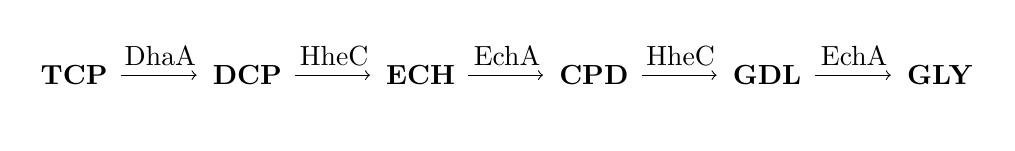
\begin{tikzpicture}[shorten >=1pt,node distance=2.2cm] %thick,>=stealth'
	\node[state] (a) [draw=none]  {$\bf TCP$};
	\node[state] (b) [right of=a,draw=none] {$\bf DCP$};
%	\node[state] (b) [above right of=a,draw=none] {$\bf R$-$\bf DCP$};
%	\node[state] (b2) [below right of=a,draw=none] {$\bf S$-$\bf DCP$};
%	\node[state] (c) [below right of=b,draw=none] {$\bf ECH$};
	\node[state] (c) [right of=b,draw=none] {$\bf ECH$};
	\node[state] (d) [right of=c,draw=none] {$\bf CPD$};
	\node[state] (e) [right of=d,draw=none] {$\bf GDL$};
	\node[state] (f) [right of=e,draw=none] {$\bf GLY$};
	\path[->]
	(a) edge  node [sloped,above] {DhaA} (b)
%	(a) edge  node [sloped,below] {DhaA} (b2)
	(b) edge  node [sloped,above] {HheC} (c)
%	(b2) edge  node [sloped,below] {HheC} (c)
	(c) edge  node [above] {EchA} (d)
	(d) edge  node [above] {HheC} (e)
	(e) edge  node [above] {EchA} (f)
;
	%(n) edge  [bend left, dashed] node {} (y);
\end{tikzpicture}\\
%	}
\vspace*{-4mm}
%{\tiny
%$$\frac{d[TCP]}{dt} = -\frac{k_1\cdot DhaA\cdot[TCP]}{K_{m,1}+[TCP]}, \ \ \frac{d[DCP]}{dt} = \frac{k_1\cdot DhaA\cdot [TCP]}{K_{m,1}+[TCP]} -\frac{k_2\cdot HheC\cdot [DCP]}{K_{m,2}+[DCP]}$$
%$$\frac{d[ECH]}{dt} = \frac{k_2\cdot HheC\cdot [DCP]}{K_{m,2}+[DCP]} - \frac{k_3\cdot EchA\cdot [ECH]}{K_{m,3}+[ECH]}, \ \ \frac{d[CPD]}{dt} = \frac{k_3\cdot EchA\cdot [ECH]}{K_{m,3}+[ECH]} - \frac{k_4\cdot HheC\cdot [CPD]}{K_{m,4}+[CPD]}$$
%$$\frac{d[GDL]}{dt} = \frac{k_4\cdot HheC\cdot [CPD]}{K_{m,4}+[CPD]} - \frac{k_5\cdot HheC\cdot [GDL]}{K_{m,5}+[GDL]}$$% \ \frac{d[GLY]}{dt} = \frac{k_5\cdot HheC\cdot [GDL]}{K_{m,5}+[GDL]}$$
%}
\parbox{0.5\textwidth}{
\small
$$\begin{array}{c@{$\,=\,$}l}
\frac{d[TCP]}{dt} & -\frac{k_1\cdot DhaA\cdot [TCP]}{K_{m,1}+[TCP]}\\[2mm]
\frac{d[DCP]}{dt} & \frac{k_1\cdot DhaA\cdot \cdot [TCP]}{K_{m,1}+[TCP]} -\frac{k_2\cdot HheC\cdot [DCP]}{K_{m,2}+[DCP]}\\[2mm]
\frac{d[ECH]}{dt} & \frac{k_2\cdot HheC\cdot [DCP]}{K_{m,2}+[DCP]} - \frac{k_3\cdot EchA\cdot [ECH]}{K_{m,3}+[ECH]}\\[2mm]
%\frac{d[CPD]}{dt} & \frac{k_3\cdot EchA\cdot [ECH]}{K_{m,3}+[ECH]} - \frac{k_4\cdot HheC\cdot [CPD]}{K_{m,4}+[CPD]}\\[2mm]
%\frac{d[GDL]}{dt} & \frac{k_4\cdot HheC\cdot [CPD]}{K_{m,4}+[CPD]} - \frac{k_5\cdot HheC\cdot [GDL]}{K_{m,5}+[GDL]}\\[2mm]
%\frac{d[GLY]}{dt} & \frac{k_5\cdot HheC\cdot [GDL]}{K_{m,5}+[GDL]}\\[2mm]
\end{array}$$
}~
\parbox{0.5\textwidth}{
\small
$$\begin{array}{c@{$\,=\,$}l}
%\frac{d[TCP]}{dt} & -\frac{k_1\cdot DhaA\cdot [TCP]}{K_{m,1}+[TCP]}\\[2mm]
%\frac{d[DCP]}{dt} & \frac{k_1\cdot DhaA\cdot \cdot [TCP]}{K_{m,1}+[TCP]} -\frac{k_2\cdot HheC\cdot [DCP]}{K_{m,2}+[DCP]}\\[2mm]
%\frac{d[ECH]}{dt} & \frac{k_2\cdot HheC\cdot [DCP]}{K_{m,2}+[DCP]} - \frac{k_3\cdot EchA\cdot [ECH]}{K_{m,3}+[ECH]}\\[2mm]
\frac{d[CPD]}{dt} & \frac{k_3\cdot EchA\cdot [ECH]}{K_{m,3}+[ECH]} - \frac{k_4\cdot HheC\cdot [CPD]}{K_{m,4}+[CPD]}\\[2mm]
\frac{d[GDL]}{dt} & \frac{k_4\cdot HheC\cdot [CPD]}{K_{m,4}+[CPD]} - \frac{k_5\cdot HheC\cdot [GDL]}{K_{m,5}+[GDL]}\\[2mm]
\frac{d[GLY]}{dt} & \frac{k_5\cdot HheC\cdot [GDL]}{K_{m,5}+[GDL]}\\[2mm]
\end{array}$$
}\\%\vspace*{-2mm}
{\scriptsize$k_1 = 1.05$, $k_2 = 0.751$, $k_3 = 14.37$, $k_4 = 2.38$, $k_5 = 3.96$,\\ $K_{m,1} = 1.79$, $K_{m,2} = 1.00$, $K_{m,3} = 0.09$, $K_{m,4} = 0.86$, $K_{m,5} = 3.54$}\\
%\hspace*{1cm}
%\parbox{0.2\textwidth} {
%\scriptsize
%$$\begin{array}{c@{$\,=\,$}l}
%k_1 & 1.05\\
%K_{m,1} & 1.79\\
%\end{array}$$
%}~
%\parbox{0.2\textwidth} {
%\scriptsize
%$$\begin{array}{c@{$\,=\,$}l}
%k_2 & 0.751\\
%K_{m,2} & 1.00\\
%\end{array}$$
%}~
%\parbox{0.2\textwidth} {
%\scriptsize
%$$\begin{array}{c@{$\,=\,$}l}
%k_3 & 14.37\\
%K_{m,3} & 0.09\\
%\end{array}$$
%}~
%\parbox{0.2\textwidth} {
%\scriptsize
%$$\begin{array}{c@{$\,=\,$}l}
%k_4 & 2.38\\
%K_{m,4} & 0.86\\
%\end{array}$$
%}~
%\parbox{0.2\textwidth} {
%\scriptsize
%$$\begin{array}{c@{$\,=\,$}l}
%k_5 & 3.96\\
%K_{m,5} & 3.54\\
%\end{array}$$
%}
\vspace*{-4.5mm}
    \end{center}
%\caption{Schematic model (left) and mathematical model (right) of n-dimensional repressilator ($Rep^n$).}
\caption{
(Up) An abstract scheme of the original system. %enzymatic chain reaction %for biodegradation of TCP to GLY. 
%Note, that enzyme DhaA produces two different forms (enantiomers) of intermediate DCP with similar rate but each has different enantioselectivity against enzyme HheC.
%Another worth noting fact is 
Note that enzymes HheC and EchA are employed twice on the pathway. The reverse mass flow is considered negligible and abstracted away. (Down) The mathematical model. Enzyme concentrations are considered as constant (and unknown) parameters. Units: $k_x (s^{-1})$, $K_{m,x} (mM)$.
}
\label{fig:enzymatic-pathway}
\vspace*{-5mm}
\end{figure}

These enzymes are  haloalkane dehalogenase (DhaA) from \emph{Rhodococcus rhodo\-chrous} and haloalcohol dehalogenase (HheC), epoxide hydrolase (EchA) from \emph{Agrobacterium radiobacter}. They have the major role in this pathway. In order to achieve an efficient implementation of the pathway it is important to quantitatively characterise mutual interplay and optimal concentration levels of these enzymes. In general, the higher is the enzyme concentration the higher is the flux rate. Especially, if a substrate and its intermediates are more or less toxic to a host cell such a requirement becomes critical. 

Unfortunately, the solution is not straightforward because each of the enzymes has a distinct rate and some of the intermediate products are much more toxic than the others. Additionally, since these enzymes are not natural proteins in \emph{E. coli}, they have to be produced at the expense of other substances. This is called \emph{metabolic burden}. In other words, there must be a balance in concentrations of these enzymes in order to degrade TCP as fast as possible while not killing the host by enervation. Therefore, we employ our workflow to answer the question on optimal enzyme concentration levels. % if we have some knowledge about the system in forward.

%{\color{red}
%In~\cite{kurumbang2013computer} the authors designed and tested three slightly different mutant forms of DhaA in order to improve an efficiency of the pathway. Nevertheless we consider just the most efficient form called DhaA31 (reffered here just as DhaA for simplicity) with associated constants $k_1$ and $K_{m,1}$ (see Fig.~\ref{fig:enzymatic-pathway}).
%}

%The original model is composed of two enantiomers of DCP formed by DhaA in almost equal amount. Unfortunately they have highly different affinity to their common catalyst (HheC). % in consequence of 
%As a result S-DCP accumulates during the process of degradation until R-DCP is consumed. Note that both enantiomers are supposed to be equally toxic to a host. Hence, we can abstract from them and consider just one substance (DCP) with particular new constants
%$$k^{'}_1 = k_0+k_1,$$$$k^{'}_2= \frac{k_2}{K_{m,2}}+\frac{k_3}{K_{m,3}},$$$$K^{'}_{m,2}=1$$
%replacing the former used in~Fig.\ref{fig:enzymatic-pathway}. 

The original model taken from~\cite{dvorak2014engineering} was reduced in order to minimise the dimensionality of the system.
Redundant reactions are eliminated based on their rates and catalytic efficiency (defined as $\frac{k_x}{K_{m,x}}$,  see Table~\ref{tab:reactions}).
%If we look at reaction rate and particular catalytic efficiency (defined as $\frac{k_x}{K_{m,x}}$) of each reaction in Table \ref{tab:reactions} an abstraction suggests itself. 
In general, greater catalytic efficiency means a faster reaction flux towards generation of the product. Since we need to preserve the number of unknown parameters, the very first reaction cannot be omitted. Reaction towards CPD is undeniably the fastest reaction of the model not just due to the best catalytic efficiency but also because of the highest affinity which is an alternative interpretation of the reciprocal Michaelis constant. Therefore this reaction can be omitted in our model. The reaction towards GDL has the second fastest flux and since it is much faster than the last reaction % and mass will accumulate 
%right before it we could also omit the one towards GDL.
 it can be omitted as well.
Finally, we have reduced the model to only three reactions which significantly helps to reduce the model state space while making the investigation of the three uncertain parameters tractable. 

\begin{table}[t]
%\vspace*{-2mm}
  \caption{Model reactions including enzymes, reaction constants and additional information about catalytic efficiency.}
  \label{tab:reactions}
 \centering
 \setlength{\tabcolsep}{5pt}
 \begin{tabular}{ |{c}|{c}|*{3}{r|} }
    \hline
	{\em reaction} & {\em enzyme} & {\em rate ($k$)} & {\em Michaelis const. ($K_m$)} & {\em cat. efficiency ($\frac{k}{K_m}$)} \\ \hline \hline
%%%% Table for: AG low || AG high
TCP$\rightarrow$DCP & DhaA & 1.050 &  1.79 &  0.587  \\ \hline
DCP$\rightarrow$ECH & HheC & 0.751 &  1.00 &  0.751  \\ \hline
ECH$\rightarrow$CPD & EchA & 14.370 & 0.09 & 159.670 \\ \hline
CPD$\rightarrow$GDL & HheC & 2.380 & 0.86 & 2.767 \\ \hline
GDL$\rightarrow$GLY & EchA & 3.960 & 3.54 & 1.119 \\ \hline
  \end{tabular}
\end{table}

The desired property is defined 
%just in verbal way 
verbally
as ``\emph{complete degradation of TCP as fast as possible with the least accumulated toxicity}''. The notion of toxicity is based on inhibitory concentration of particular molecules. % and defined as \oprav{a sum of relative values per actual concentration of each molecule}. 
Our framework
%is not suitable for manipulation with numerical assignments. 
is designed for manipulation with differential expressions rather than with numerical assignments. 
Hence we are not able to directly observe actual amount of toxicity.
But the toxicity has a direct connection to the concentrations of intermediates. To this end, we translate the desired property as ``\emph{TCP completely degrades and the concentration of intermediates does not exceed given bounds}''. The bounds are based on experimental data of the original model (Fig.~\ref{fig:simulation-default}) with the default setting of parameters (DhaA $=0.003$, HheC $=0.0036$, EchA $=0.0029$ $(mM)$) and initial concentrations ($[TCP] = 2 \ mM$, $[other \ species]=0 \ mM$). Constants are shown in Fig.~\ref{fig:enzymatic-pathway}. The presented data reveal that the considered boundary is reasonable for the concentration $0.5 \ mM$ or less.
%These bounds are unknown so far therefore we need to exploit some simulation tool. For this particular case the Biocham \cite{calzone2006biocham} was used with the initial conditions of concentrations ($[TCP] = 2 \ mM$, $[other \ species]=0 \ mM$) and the default setting of parameters according to \cite{kurumbang2013computer} (constants are defined in Fig.~\ref{fig:enzymatic-pathway}). The figure \ref{fig:simulation-default} reveals that such boundary is reasonable for the concentration of $0.5 \ mM$ or less.
In consequence, we proceed by testing various combinations of bounds for GDL and DCP in the interval $[0,0.5]$ of $mM$.
\enlargethispage*{7mm}

\begin{figure}
\center
\includegraphics[scale=0.4]{experiment_1.png}
\caption{Experimental data from the original model~\cite{kurumbang2013computer}. We are interested just in the progress of TCP, DCP, GDL and GLY taken as variables of our reduced model. Note the time scale and the maximal reached concentration of DCP and GDL.
%Numerical simulation of the reduced model (biodegradation of TCP) obtained by Biocham tool for parameter setting: $DhaA=0.003$, $HheC=0.0036$, $EchA=0.0029$ $(mM)$.
%Time duration of simulation was set according to~\cite{kurumbang2013computer} to 5 hours.
%Note the maximal reached concentration of intermediate products DCP and GDL.
}
\label{fig:simulation-default}
\end{figure}

It has been mentioned that concentration of enzymes cannot be unlimited due to the metabolic burden (which is not the object of investigation in this paper). According to the default values 
% ($DhaA=0.003$, $HheC=0.0036$, $EchA=0.0029$ $(mM)$) 
the initial constraints for these parameters are therefore set to the interval $[0.0,0.02]$ of $mM$. The parameter synthesis workflow is employed in order to find parameter values satisfying the desired property. 
The template of CTL formula expressing the property (denoted as $\varphi$) %(let denote it $\varphi$)  
is a combination of several smaller subformulae:


{\scriptsize $$\varphi_1 = ({\bf AG}\ [TCP]<y), \ \ \varphi_2 = ({\bf A}([TCP]>x){\bf U}({\bf AF}\ \varphi_1)),$$
%$$\varphi_2 = ({\bf A}([TCP]>1.9){\bf U}({\bf AF}\ \varphi_1)),$$
$$\varphi_3 = ({\bf AG}\ [GLY]>x), \ \ \varphi_4 = ({\bf A}([GLY]<y){\bf U}({\bf AF}\ \varphi_3)),$$
%$$\varphi_4 = ({\bf A}([GLY]<0.01){\bf U}({\bf AF}\ \varphi_3)),$$
$$\varphi_6 = ({\bf AG}\ [DCP]<v), \ \ \varphi_7 = ({\bf AG}\ [GDL]<w),$$
%$$\varphi_7 = ({\bf AG}\ [GDL]<w),$$
$$\varphi_5= (\varphi_2 \land \varphi_4),\ \ \varphi_8 = (\varphi_5 \land \varphi_6), \ \ \varphi = (\varphi_8 \land \varphi_7),$$}%
%can be represented by template:
%$$(([TCP]>x) \text{AU} (\text{AF AG} \ [TCP]<y)) \land (([GLY]<y)\text{AU}(\text{AF AG} \ [GLY]>x))...$$\\
%$$...\land (\text{AG} \ [DCP]<v) \land (\text{AG}\ [GDL]<w),$$
where $x$, $y$, $v$ and $w$ are estimated values making a particular instance of this property. 
%In this case study we use 
Here %, it is used
$x=1.9$ (according to \cite{kurumbang2013computer} where authors use the value 2 $mM$), $y=0.01$ (cannot be zero), $v\in\{0.5,0.3,0.1\}$ and $w\in\{0.5,0.25,0.1\}$ (variations based on an observation of the experimental data in Fig.~\ref{fig:simulation-default}).

The resulting formula is quite large. However, due to the global nature of enumerative CTL model checking algorithm all the subformulae are investigated during the process. %(Table~\ref{tab:satisfying-states})
This feature can be very convenient in many cases. The computation took 
more than one day on one computing node while  
less than 2 hours on twenty nodes (each node equipped with common HW -- Intel Xeon quad-core 2GHz and 16 GB of RAM).

%The precision of the PMA approximation of the model has been set to the following numbers of discretising thresholds considered for the respective model variables (the numbers are in the form {\em explicit + implicit}): TCP ($7+5$), DCP ($10+5$), GDL ($8+5$), GLY ($5+0$). Explicit thresholds are defined manually and are based on experimental observation. Implicit thresholds are generated automatically by the approximation procedure. There is no implicit threshold defined for GLY because no sigmoidal function in the model depends on GLY.
%{\color{red}designed for a transformation of the non-linear functions (such as Michaelis-Menten's) into the piecewise affine functions up to some error value}
%(Sec.~\ref{sec:methods}).

%Regardless of 
%%concrete values of variables and parameters 
%specific instantiation
%the model has been set up such that transition-state space of size 2688 states is obtained. By set up it is meant the number of  explicit and implicit 
%%(a result of optimal linear approximation) 
%thresholds which the rectangular abstraction
%%\cite{Batt2007} 
%depends on (Sec.~\ref{sec:methods}). While the explicit thresholds are user-defined and based on an experimental observation or a wide experience the implicit thresholds are the product of the optimal linear approximation {\color{red}(defined in~\cite{GrosuBFGGSB11})} designed for a transformation of the non-linear functions (such as Michaelis-Menten's or Hill's) into the piecewise affine functions up to some error value. 
%%The relatively small number of states is compensation for quite big property need to be verified. However, due to the nature of CTL model checking algorithm all subformulae has been investigated during the process (see Table~\ref{tab:satisfying-states}). Such feature can be very convenient in many cases. It took almost 68 hours on one computational node while less than  2 hours on twelve nodes.

%\begin{table}[t]
% \caption{Numbers of states satisfying a particular CTL (sub)formula (defined above) for various combinations of $v$ and $w$. 
%  %$\varphi_1 = (\text{AG} \ [TCP]<0.01)$; $\varphi_2 = (([TCP]>1.9) \text{AU} (\text{AF }\varphi_1))$; $\varphi_3 = (\text{AG} \ [GLY]>1.9)$; $\varphi_4 = (([GLY]<0.01)\text{AU}(\text{AF }\varphi_3))$; $\varphi_5= (\varphi_2 \land \varphi_4)$; $\varphi_6 = (\text{AG} \ [DCP]<v)$; $\varphi_7 = (\varphi_5 \land \varphi_6)$; $\varphi_8 = (\text{AG}\ [GDL]<w)$ and $\varphi_9 = (\varphi_7 \land \varphi_8)$.
%  }
%  \label{tab:satisfying-states}
% \centering
% \setlength{\tabcolsep}{5pt}
% \begin{tabular}{ |{c}|*{9}{r|} }
%    \hline
%	($v,w$) & $\varphi_1$ & $\varphi_2$ & $\varphi_3$ & $\varphi_4$ & $\varphi_5$ & $\varphi_6$ & $\varphi_7$ & $\varphi_8$ & $\varphi$  \\ \hline \hline
%%%% Table for: AG low || AG high
%(0.5,0.5) & 672 & 672 & 336 & 672 & 168 & 1344 & 2304 & 84 & 72 \\ \hline
%(0.5,0.25) & 672 & 672 & 336 & 672 & 168 & 1344 & 1536 & 84 & 48 \\ \hline
%(0.5,0.1) & 672 & 672 & 336 & 672 & 168 & 1344 & 1152 & 84 & 36 \\ \hline
%(0.3,0.1) & 672 & 672 & 336 & 672 & 168 & 896 & 1152 & 56 & 24 \\ \hline
%[0.2,0.1] & 672 & 672 & 336 & 672 & 168 & 896 & 56 & 1152 & 24 \\ \hline
%(0.1,0.1) & 672 & 672 & 336 & 672 & 168 & 896 & 1152 & 56 & 24 \\ \hline
%  \end{tabular}
%\end{table}

The result of parameter synthesis is the set of initial states (satisfying $\varphi$) each accompanied with a set of respective values of the parameters (DhaA, HheC, EchA). Results are encoded as a formula in the SMT-LIB format 2.5~\cite{smtlib25}. %(Fig.~\ref{fig:example-of-formula}). 
Consequently, to compare and visualise satisfactory parameter values in a human-readable form 
%the obtained results can be post-processed in various ways.
some post-processing is necessary. In this case, we run a script that systematically samples and visualises the parameter space encoded by the formula (by calling the SMT solver iteratively). The result is the graphical representation of the parameter subspace constraint by $\varphi$ and the initial parameter constraints. In Fig.~\ref{fig:damborsky-param-space} the results are shown for a specific initial state. 

% \begin{figure}
% \scriptsize
% %\center
% \hspace*{2cm}(and ($<$= (+ (* (/ 5816875963663419.0 25000000000000000.0) HheC)\\
% \hspace*{3.64cm}            (* (- (/ 5324431169167469.0 500000000000000.0)) EchA))\\ 
% \hspace*{3.25cm} 0.0)\\
% \hspace*{2.56cm}     ($<$= (+ (* (/ 5486128154511019.0 10000000000000000.0) DhaA)\\
% \hspace*{3.64cm}            (* (- (/ 5816875963663419.0 25000000000000000.0)) HheC))\\
% \hspace*{3.25cm} 0.0)\\
% \hspace*{2.56cm}     (not ($<$= DhaA 0.0))\\
% \hspace*{2.56cm}     (not ($<$= (/ 1.0 50.0) HheC))\\
% \hspace*{2.56cm}     (not ($<$= (/ 1.0 50.0) EchA)))
% \caption{The simple example of a resulting formula constraining parameter space in a particular initial state obtained from our framework in the SMT-LIB format~\cite{smtlib25}. 
% %Parameters p0, p1 and p2 stand for DhaA, HheC and EchA respectively.
% }
% \label{fig:example-of-formula}
% \end{figure}

%{\color{red}
% One of them is solving a formulae in specific conditions (i.e., points in the parameter space) and other one is introduced in the next case study. An exact result could be obtained in this way (as an answer for a satisfiability question in a particular point). Accordingly, a bunch of such points could be  sampled and visualized for one formula as well as for a set.
% %more combined together. 
% We employ a script in R language to do that and the outcome  represents parameter subspace constrained 
% w.r. to $\varphi$. }
%for meeting the property $\varphi$.  

%{\color{red} pridat definiciu alebo zdovodnenie pre nejaky {\em celkovy}  param. priestor ako zjednotenie cez vsetky splnajuce inic. podmienky}
%{\color{red} dalej by bolo fajn porovnat s vysledkami funkcie landscape BIOCHAMu. Obrazok z vyhovujucej oblasti, z nevyhovujucej oblasti a z hranicnej oblasti. Pripadne num. simulacie priebehu v tych parametrizaciach.}
%There were too many of states satisfying the reachability of both equilibria for providing a table. However, parameter constraints meeting this property are pictured with {\em green} color beside the parameter settings for the {\em low} (with {\em blue}) and the {\em high} (with {\em red}) stable states (Fig. \ref{fig:tcbb-param-space}).

\begin{figure}[!h]
\center
\begin{overpic}[width=0.42\textwidth]{damborsky_3D_state3.png}
\put(48,3){\scriptsize \bf DhaA}
\put(70,15){\scriptsize \bf HheC}
\put(77,50){\scriptsize \bf EchA}
\end{overpic} \hspace*{5mm}
\begin{overpic}[width=0.45\textwidth]{damborsky_2D_p0_p1_state3.png}
\put(48,1.5){\scriptsize \bf DhaA}
\put(2,38){\scriptsize \bf \rotatebox{90}{HheC}}
\end{overpic}\\
\begin{overpic}[width=0.45\textwidth]{damborsky_2D_p0_p2_state3.png}
\put(48,1.5){\scriptsize \bf DhaA}
\put(2,38){\scriptsize \bf \rotatebox{90}{EchA}}
\end{overpic}\hspace*{1mm}
\begin{overpic}[width=0.45\textwidth]{damborsky_2D_p1_p2_state3.png}
\put(48,1.5){\scriptsize \bf HheC}
\put(2,38){\scriptsize \bf \rotatebox{90}{EchA}}
\end{overpic}
\caption{A sample of the resulting parameter space for a particular initial state: TCP $\in[1.9,1.9586]$, DCP $\in[0.448898,0.5]$, GDL $\in[0.0,0.0669138]$, GLY $\in[0.0,0.01]$. Dotted area corresponds to  $\varphi$ ($v = 0.5$, $w=0.25$).
%$(([TCP]>1.9) \text{AU} (\text{AF AG} \ [TCP]<0.01)) \land (([GLY]<0.01\text{AU}(\text{AF AG} \ [GLY]>1.9)) \land (\text{AG} \ [DCP]<0.5) \land (\text{AG}\ [GDL]<0.25)$.
%Parameters $p_0$, $p_1$ and $p_2$ stand for DhaA, HheC and EchA respectively. 
(Up left figure) The 3D space sampled with 400 points per a layer. (Other figures) Projection of the 3D plot for every combination of unknown parameters. All values are shown in $mM$.
%This particular parameter constraints satisfy the above property for initial state: $TCP\in[1.9,1.9586], DCP\in[0.448898,0.5], GDL\in[0.0,0.0669138], GLY\in[0.0,0.01]$.
}
\label{fig:damborsky-param-space}
\vspace*{-3mm}
\end{figure}

Finally, we further process the obtained parameter values by numerical simulation in order to evaluate the validity of $\varphi$ in the original model (Fig.~\ref{fig:simulations}). Some points of the resulting parameter space (Fig.~\ref{fig:damborsky-param-space} (up left)) were selected as representatives of the satisfiable, unsatisfiable and {\em in-between} area. By {\em in-between} it is meant the layer of points very close to satisfiable area but still being unsatisfiable. Since we operate on an overapproximated system, the result represents an underapproximation of the exact solution. Hence the points in the {\em in-between} area might satisfy a given property in the original ODE model even though our framework has refused them. 

\begin{figure}
\centering
\begin{overpic}[width=\textwidth]{simulations_together.png} % sat | in-betw | unsat | unsat
\put(45,-0.5){\scriptsize Time (s)}
\put(0,18){\scriptsize \rotatebox{90}{Concentration ($mM$)}}
\put(2.2,53.5){\tiny$2.5$}\put(2.2,49.5){\tiny$2.0$}\put(2.2,45.5){\tiny$1.5$}\put(2.2,41.5){\tiny$1.0$}\put(2.2,37.5){\tiny$0.5$}\put(2.2,33.5){\tiny$0.0$}%\put(2.2,29.5){\tiny$-0.5$}
\put(2.2,28.5){\tiny$2.5$}\put(2.2,24.5){\tiny$2.0$}\put(2.2,20.5){\tiny$1.5$}\put(2.2,16.5){\tiny$1.0$}\put(2.2,12.5){\tiny$0.5$}\put(2.2,8.5){\tiny$0.0$}
\put(4.5,3){\tiny \rotatebox{40}{0}}\put(7.5,1.2){\tiny \rotatebox{40}{1000}}\put(12.5,1.2){\tiny \rotatebox{40}{2000}}\put(17.7,1.2){\tiny \rotatebox{40}{3000}}\put(22.9,1.2){\tiny \rotatebox{40}{4000}}\put(28.0,1.2){\tiny \rotatebox{40}{5000}}\put(33.2,1.2){\tiny \rotatebox{40}{6000}}\put(38.3,1.2){\tiny \rotatebox{40}{7000}}\put(43.5,1.2){\tiny \rotatebox{40}{8000}}\put(48.7,1.2){\tiny \rotatebox{40}{9000}}
\put(52.2,3){\tiny \rotatebox{40}{0}}\put(55.1,1.2){\tiny \rotatebox{40}{1000}}\put(60.2,1.2){\tiny \rotatebox{40}{2000}}\put(65.3,1.2){\tiny \rotatebox{40}{3000}}\put(70.45,1.2){\tiny \rotatebox{40}{4000}}\put(75.6,1.2){\tiny \rotatebox{40}{5000}}\put(80.75,1.2){\tiny \rotatebox{40}{6000}}\put(85.9,1.2){\tiny \rotatebox{40}{7000}}\put(91,1.2){\tiny \rotatebox{40}{8000}}\put(96.2,1.2){\tiny \rotatebox{40}{9000}}
\put(7.5,47){\tiny TCP}\put(18,47){\tiny GLY}\put(12,35.5){\tiny DCP}\put(12,32.8){\tiny GDL}
\put(54,47){\tiny TCP}\put(64,47){\tiny GLY}\put(53,38){\tiny DCP}\put(56,34){\tiny GDL}
\put(5.5,23){\tiny TCP}\put(25,22){\tiny GLY}\put(13,20){\tiny DCP}\put(13,9.2){\tiny GDL}
\put(53.2,23){\tiny TCP}\put(58.4,23){\tiny GLY}\put(56.5,11.5){\tiny DCP}\put(53.1,7.1){\tiny GDL}
\end{overpic}
\vspace*{-5mm}
\caption{Numerical simulations for particular parameter values obtained as the outcome of our framework. (Up left) Satisfiable configuration: DhaA = 0.0015, HheC = 0.007, EchA = 0.01. (Up right) {\em In-between} configuration: DhaA = 0.0035, HheC = 0.005, EchA = 0.005. (Down left) Unsatisfiable configuration: DhaA = 0.01, HheC = 0.001, EchA = 0.01. (Down right) Unsatisfiable configuration: DhaA = 0.01, HheC = 0.01, EchA = 0.01. All values are in $mM$. Simulations were obtained in BIOCHAM~\cite{RBF+09}.}
\label{fig:simulations}
\vspace*{-4mm}
\end{figure}

%It is worth mentioning 
Note that due to the global nature of our algorithm  
%which find all satisfying initial states
all states satisfying the property have been found.
%our framework for this case study, with 
Concentration of all variables in this case study has been restricted to the interval $[0.0,5.0]$ $mM$. Our framework reveals parameter values satisfying $\varphi$ also for initial states beyond the singular initial concentration of particular species considered in \cite{kurumbang2013computer}. The most interesting are the initial states that increase the upper limit of TCP concentration wrt $\varphi$ (Fig.~\ref{fig:expanded-inits}). 

\begin{figure}[t]
\centering
\begin{overpic}[width=0.4\textwidth]{param_space_for_expanded_inits.png}
\put(12,5){\scriptsize\bf DhaA}
\put(82,5){\scriptsize\bf HheC}
\put(82,53){\scriptsize\bf EchA}
\end{overpic} \hspace*{2mm}
\begin{overpic}[width=0.55\textwidth]{expanded_init_states_dhaa=0001_hhec=0005_echa=0015_2.png}
\put(45,-1){\scriptsize Time (s)}
\put(-1.5,12){\scriptsize \rotatebox{90}{Concentration ($mM$)}}
\put(3,53.5){\tiny$4.5$}\put(3,49){\tiny$4.0$}\put(3,44.5){\tiny$3.5$}\put(3,40){\tiny$3.0$}\put(3,35.5){\tiny$2.5$}\put(3,31){\tiny$2.0$}\put(3,26){\tiny$1.5$}\put(3,21){\tiny$1.0$}\put(3,16.6){\tiny$0.5$}\put(3,12){\tiny$0.0$}

\put(7,5){\tiny \rotatebox{30}{0}}\put(13,2.2){\tiny \rotatebox{30}{2000}}\put(23,2.2){\tiny \rotatebox{30}{4000}}\put(33,2.2){\tiny \rotatebox{30}{6000}}\put(43.2,2.2){\tiny \rotatebox{30}{8000}}\put(51.5,2){\tiny \rotatebox{30}{10000}}\put(61.5,2){\tiny \rotatebox{30}{12000}}\put(71.5,2){\tiny \rotatebox{30}{14000}}\put(81.5,2){\tiny \rotatebox{30}{16000}}\put(91.5,2){\tiny \rotatebox{30}{18000}}

\put(15,42){\tiny TCP}\put(42,42){\tiny GLY}\put(18,15){\tiny DCP}\put(18,10.2){\tiny GDL}
\end{overpic}
\caption{(Left) Resulting parameter space for a specific initial state: TCP $\in[3.84186,5.0]$, DCP $\in[0.0,0.448898]$, GDL $\in[0.0,0.0669138]$, GLY $\in[0.0,0.01]$. The red dot shows the selected point for parameters values: DhaA = 0.001, HheC = 0.005, EchA = 0.015. (Right) Numerical simulation for the selected point. All values are in~$mM$. Simulation was obtained in BIOCHAM~\cite{RBF+09}.
}
\label{fig:expanded-inits}
\vspace*{-4mm}
\end{figure}

%Or by involving some SMT-based optimiztion tool like Symba~\cite{Li15} to obtain
%an approximated interval of the bounds on valid parameter values. %(Table \ref{tab:tcbb-bistab-table} ($2^{nd}$ and $3^{rd}$ column)). 
%This kind of data is simple and user-friendly, however, since the considered parameters are in linear dependency the results cannot be simply combined to display the two-dimensional validity area in the parameter space. To this end, additional information about the parameter ratio need to be employed. %(Table \ref{tab:tcbb-bistab-table} ($4^{th}$ column)). 
%This could be handled by the same tool. Therefore this information is also provided as an interval but this time guaranteed due to the very same linear dependency. By combination the parameter bounds with a parameter ratio interval an exact parameter subspace is acquired up to the guarancy of our model checking procedure. Of course, the results look very similar to the previous one  since they are projection-like figures for different layers of 3D plot (Fig.~\ref{fig:tcbb-param-space}).

\enlargethispage*{4mm}
\subsection{Regulation of $\bf G_1 / S$ cell cycle transition}

This case study is focused on extension of previous analysis from~\cite{CMSB15} of the model describing regulatory interactions controlling a transition between two phases of a mammalian cell cycle~\cite{SKH04}. In particular, the model explains the core mechanism behind the irreversible decision for cell division described by a two-gene regulatory network of interactions between the tumour suppressor protein $pRB$ and the central transcription factor $E2F1$ (Fig.~\ref{fig:genmodel} (left)). For suitable parameter values, two distinct stable attractors may exist (the so-called \emph{bistability}). In~\cite{SKH04} a numerical bifurcation analysis of $E2F1$ stable concentration depending on the degradation parameter of $pRB$ ($\phi_{pRB}$) has been provided. Note that traditional methods for bifurcation analysis hardly scale to more than a single model parameter.

\begin{figure}[b]
\vspace*{-7mm}
  \begin{center}
\hspace*{-6mm}\parbox{3.8cm}{\includegraphics[scale=.7]{gs1net.pdf}}~\hspace*{6mm}
\parbox{6.7cm}{
\scriptsize
$$\begin{array}{c@{$\,=\,$}l}
\frac{d[pRB]}{dt} & k_1 \frac{[E2F1]}{K_{m1}+[E2F1]}\frac{J_{11}}{J_{11}+[pRB]}  - \phi_{pRB}[pRB]\\[1mm]
\frac{d[E2F1]}{dt} & k_p + k_2 \frac{a^2+[E2F1]^2}{K_{m2}^2+[E2F1]^2}\frac{J_{12}}{J_{12}+[pRB]} - \phi_{E2F1} [E2F1]
\end{array}$$
$a = 0.04$, $k_1=1$, $k_2=1.6$, $k_p=0.05$, $\phi_{pRB}=0.005$ \\$\phi_{E2F1}=0.1$, $J_{11}=0.5$, $J_{12}=5$, $K_{m1}=0.5$, $K_{m2}=4$\\
}\\
    \end{center}
    \vspace*{-4mm}
\caption{$G_1/S$ transition regulatory network (left) and its ODE model (right).}
\label{fig:genmodel}
\end{figure}

In this paper we demonstrate that by employing our algorithm we can provide bifurcation analysis for more than one parameter.
%We demonstrate that our algorithm can overcome main drawbacks of numerical methods. In particular, 
In particular, we focus on the synthesis of values of two interdependent parameters. We show how the new results complement the results obtained with the algorithm employing the interval-based representation of mutually independent parameters~\cite{CMSB15}. Additionally, we compare the results achieved within our workflow with the numerical analysis provided in~\cite{SKH04}. 

The property of {\em bistability} expresses that the system is able to settle in two distinct stable states (i.e., levels of concentration) for specific initial conditions and particular parameter values. It implies existence of a decision-making point (or area) in the system. %In some fields of study also called a {\em bifurcation point}. The decision is dependent on many other factors which are not considered here hence it is supposed to be undeterministic. %for our case.

The main outcome of the original analysis is shown in Figure~\ref{fig:bifurcation-analysis} (left) (produced by numerical analysis) displaying the dependency of stable concentration of $E2F1$ on value of $\phi_{pRB}$ (degradation rate). The most interesting area called {\em unstable} (for $\phi_{pRB} \in [0.007,0.027]$) 
%imposes horizontal range on x-axis which 
determines feasible values of $\phi_{pRB}$ wrt the above property.  For $\phi_{pRB}<0.007$ the system converges to a lower-concentration stable equilibrium whereas for
%values of 
$\phi_{pRB}>0.027$ it converges to a higher-concentration stable equilibrium.

\begin{figure}
\begin{overpic}[width=0.49\textwidth]{bifurcation_analysis.png}
\put(2,30){\scriptsize \rotatebox{90}{$E2F1$}}
\put(45,0){\scriptsize $\phi_{pRB}$}
\end{overpic} \hspace*{2mm}
\begin{overpic}[width=0.47\textwidth]{cmsb_2015_result_2.png}
\put(1,35){\scriptsize  \rotatebox{90}{$E2F1$}}
\put(45,0){\scriptsize  $\phi_{pRB}$}
\end{overpic}
\vspace*{-1mm}
\caption{(Left) Equilibrium curve for $E2F1$ in proportion to $\phi_{pRB}$ as the result of bifurcation analysis~\cite{SKH04} (the authors confirmed the scale of $\phi_{pRB}$ in the figure should be $0.005$-$0.035$ according to the text). (Right) Model checking results. Red and blue are the $high$ and $low$ stable regions, respectively. Yellow are the states where $\varphi_1$ holds.}
\label{fig:bifurcation-analysis}
\vspace*{-2mm}
\end{figure}

The CTL representation of the property in consideration is
$\varphi_1 = (\EF[\AG[low]]$ ${}\land \EF[\AG[high]])$ where $low = (0.5 < E2F1 < 2.5)$ (representing safe cell behaviour) and $high = (4 < E2F1 < 7.5)$ (representing excessive cell division). During the single run of our algorithm all subformulae of $\varphi_1$ have been analysed. Let $\varphi_2 = (\AG[low])$ and $\varphi_3 = (\AG[high])$ as the most interesting.

In~\cite{CMSB15} we have investigated perturbations of a single parameter $\phi_{pRB}$ with the initial constraint $\phi_{pRB} \in [0.001,0.025]$. According to the section~\ref{sec:methods} we have first created the PMA approximation of the original ODE model (Fig.~\ref{fig:genmodel} (right)) by approximating each non-linear function in the right-hand side of ODEs with a sum of optimal sequence of piecewise affine ramp functions (the precision has been set to $70$ automatically generated segments per each non-linear function). For such a~setting the verification process took less than 10 seconds on twenty nodes.
The results were processed by a Python script 
%as it can be seen in the Figure
(Fig.~\ref{fig:bifurcation-analysis} (right)). The plot intentionally depicts the same space as the Figure~\ref{fig:bifurcation-analysis} (left) to 
%shed light upon the similarity 
show obvious similarities of these results. %In Figure~\ref{fig:bifurcation-analysis} (right) 
The blue area stands for stable concentration of $E2F1$ ($y$-axis) with particular value of $\phi_{pRB}$ ($x$-axis) satisfying the property $\varphi_2$, whereas the red area satisfies the property $\varphi_3$. The yellow area (in the middle) stands for possibility of reaching both stable concentrations. 
%{\color{red}
Due to mixing of existential and universal quantifiers (see Sec.~\ref{sec:methods}), the results achieved for $\varphi_1$ cannot be exactly interpreted. On the contrary, the results for $\varphi_2$ and $\varphi_3$ are guaranteed due to the conservativeness of the abstraction. % (Sec.~\ref{sec:methods}). 
%Our answer to the question of satisfiability of $\varphi_1$ is clearly a subset of the bifurcation analysis answer due to the overapproximation character of rectangular abstraction.
%}

Although the algorithm based on interval-based encoding performs fast, it is limited to independent parameters only. To overcome this limitation, we have employed the SMT-based algorithm to explore two uncertain mutually dependent parameters. The method is computationally more demanding (about one order of magnitude for each pair of dependent parameters). The goal of our extended analysis is to explore the mutual effect of the degradation parameter of $pRB$ ($\phi_{pRB}$) and the production parameter of $pRB$ ($k_1$) on the bistability. Additionally, we perform post-processing of achieved results by employing additional constraints on the parameter space (e.g., imposing a lower and upper bound on the production/degradation parameter ratio) and show an alternative way of presenting the results.

% {\color{red}
In particular, we involve the~SMT-based tool Symba~\cite{LiA15} to obtain
%The SMT representation of computed parameter constraints is further processed by Symba tool~\cite{Symba} to obtain
an approximated interval of the bounds on valid parameter values. %(Table \ref{tab:tcbb-bistab-table} ($2^{nd}$ and $3^{rd}$ column)).
%This kind of data is simple and user-friendly. However, 
Since the considered parameters are linearly dependent, the resulting intervals cannot be simply combined to display the two-dimensional validity area in the parameter space. To this end, we employ Symba to explore the ratio of the two parameters. %(Table \ref{tab:tcbb-bistab-table} ($4^{th}$ column)).
%This could be handled by the same tool.
% Therefore this information is also provided as an interval but this time guaranteed due to the very same linear dependency.} 
By combining initial parameter constraints with the bounds on the parameter ratio, a more accurate parameter subspace is acquired. Such an outcome has been used with the initial constraint $\phi_{pRB} \in [0.001,0.1]$ and $k_1 \in [0.001,10]$ (Fig.~\ref{fig:tcbb-ratio} (up left)). Additionally, we have explored a refined parameter space ($\phi_{pRB} \in [0.001,0.025]$ and $k_1 \in [0.001,2]$) where a one-dimensional projection on the $\phi_{pRB}$-axis is highlighted for $k_1 \approx 1$, the default value of $k_1$~(Fig.~\ref{fig:tcbb-ratio} (up right)).
%Of course, the results look very similar to the previous one  since they are projection-like figures for different layers of 3D plot (Fig.~\ref{fig:tcbb-param-space}).

\begin{figure}[t]
\begin{overpic}[width=0.49\textwidth]{tcbb_ratio_yellow.png}
%\includegraphics[scale=0.21]{tcbb_ratio_yellow.png}
\put(0,21){\scriptsize$\bf k_1$}
\put(49,1){\scriptsize$\bf \phi_{pRB}$}
\end{overpic}~
\begin{overpic}[width=0.49\textwidth]{tcbb_ratio_zoomed_2_yellow.png}
%\includegraphics[scale=0.21]{tcbb_ratio_zoomed_2_yellow.png}
\put(0,21){\scriptsize$\bf k_1$}
\put(49,1){\scriptsize$\bf \phi_{pRB}$}
\end{overpic}
\begin{overpic}[width=\textwidth]{landscape_together.png}
\put(0.5,19){\scriptsize$\bf k_1$}
\put(70,0.5){\scriptsize$\bf\phi_{pRB}$}
\put(25,0.5){\scriptsize$\bf\phi_{pRB}$}
\end{overpic}
\vspace*{-3mm}
\caption{(Up left) The resulting parameter space merged for all initial concentrations. Each area corresponds to a different property: $\varphi_1$ (yellow), $\varphi_2$ (blue) and  $\varphi_3$ (red).  (Up right) The same parameter space magnified and projected to $\phi_{pRB}$-axis. The framed region agrees with the original numerical bifurcation analysis performed in~\cite{SKH04} for $\phi_{pRB}$. (Down) Landscapes of the parameter space according to the quantitative satisfaction degree computed by BIOCHAM for $\varphi_2$ (left) and $\varphi_3$ (right), respectively.}
\label{fig:tcbb-ratio}
\vspace*{-2mm}
\end{figure}

%\begin{figure}
%\center
%\includegraphics[scale=0.23]{landscape_together.png}
%\caption{Landscapes of parameter space according to quantitative satisfaction degree for property $\varphi_2$ (left) and $\varphi_3$ (right), respectively.
%}
%\label{fig:landscape}
%\end{figure}

%\begin{figure}
%\center
%\begin{overpic}[width=\textwidth]{landscape_together.png}
%\put(0.5,19){\scriptsize$\bf k_1$}
%\put(70,0.5){\scriptsize$\bf\phi_{pRB}$}
%\put(25,0.5){\scriptsize$\bf\phi_{pRB}$}
%\end{overpic}
%\vspace*{-6mm}
%\caption{Landscapes of the parameter space according to the quantitative satisfaction degree computed by BIOCHAM for $\varphi_2$ (left) and $\varphi_3$ (right), respectively.}
%\label{fig:landscape}
%\vspace*{-2mm}
%\end{figure}

The analysis took 8 minutes on twenty nodes (excluding post-processing). 
The obtained results can be used as a base for further analysis. We employ the feature of BIOCHAM~\cite{calzone2006biocham} to compute the {\em landscape} function that allows investigation of quantitative satisfaction degree of the properties explored (Fig.~\ref{fig:tcbb-ratio} (down)). %Based on the results for properties $\varphi_2$ and $\varphi_3$ it is clear, that initial concentrations do not make a difference in this case study but the obtained boundaries for parameters are usefull. An 
LTL reformulation of $\varphi_2$ and $\varphi_3$ has been used ($\varphi_1$ cannot be expressed in LTL). The lighter is the colour the higher the satisfaction degree. 


\enlargethispage*{7mm}
\section{Conclusions}
\label{sec:conclusion}

Recently developed methods for parameter synthesis of piecewise multi-affine systems have been embedded into a general workflow for biological models. The workflow has been applied to a kinetic model of a synthetic metabolic pathway and to a model of biological switch. In the former case, we have predicted admissible configurations of required enzymes concentration that guarantee the desired production of glycerol under elimination of the toxicity. In the latter case, we have obtained computationally efficient analysis of bistability for two mutually dependent parameters. In contrast to our previous results on synthesis of independent parameters, computational loads were significantly increased. However, the parallel algorithm was able to provide the results still in reasonable times provided that an exhaustive amount of information about the systems dynamics has been computed.    

The main advantage is the global view of the systems dynamics. A disadvantage is the need for approximation and abstraction of the original ODE model. For future work, it is important to integrate the results with the approximation error and to make abstraction sensitive to the properties analysed. 


\bibliographystyle{splncs03}
\bibliography{bibliography}

\end{document}

%http://journals.plos.org/plosone/article?id=10.1371/journal.pone.0110261

% Local Variables:
% TeX-parse-self: t
% TeX-auto-save: t
% TeX-command-default: "PdfLaTeX"
% End:
